\documentclass[12pt, french]{report}
\usepackage[utf8]{inputenc}
\usepackage[T1]{fontenc}
\usepackage{babel}


%additional packages
\usepackage{amsmath}
\usepackage{lipsum}
\usepackage{graphicx}
\usepackage{caption}
\usepackage{subcaption}
\usepackage{longtable}
\graphicspath{{figures/}}
\usepackage[a4paper,width=160mm,top=25mm,bottom=25mm]{geometry}
\usepackage{titlesec}
\linespread{1.2}

\usepackage{amsfonts,epsfig,cite,array,multirow,graphicx,amsmath,amsthm,ltablex,tabularx,setspace,arydshln,amssymb,multirow}
\usepackage{schemabloc,tikz}
\usetikzlibrary{circuits, arrows}

\newtheorem{theorem}{Theorem}
\newtheorem{lemma}{Lemma}
\usepackage[utf8]{inputenc}
\usepackage{amsmath}
\usepackage{amsfonts}
\usepackage{amssymb}
\usepackage{bbm}
\usepackage{mathtools}
\usepackage{textcomp}
\usepackage{stackengine}
\usepackage{booktabs}
\usepackage{longtable}
\usepackage{multirow}
\usepackage{graphicx}
\usepackage{epigraph}
\usepackage{minitoc}
\usepackage{blindtext}
\usepackage{url}
\usepackage[hidelinks]{hyperref}
\usepackage{float}



\title{
  \LARGE{IST Deep Learning Workshop} \\
  \Large{Urdu Character recognition dataset for MLP}
}

\author{Adjimon VITOFFODJI}
\date{Juin 2025}
\def\mytitle{Challenge Kaggle }
\def\myname{Adjimon VITOFFODJI}
\def\degree{Master}
\def\mydegree{Mathématiques et Informatiques Appliqués aux Sciences Humaines et Sociales}
\def\mysupervisor{Sophie Lèbre}
\def\myrollno{17EE010XX}
\def\mydep{UPVM}



\begin{document}

%Front Matter
\dominitoc
\pagenumbering{roman}

% !TEX root = manuscript.tex
\begin{minipage}{.4\textwidth}
\begin{center}

\includegraphics[height=3cm]{logos/master.pdf}
\end{center}
\end{minipage}% This must go next to `\end{minipage}`
\hspace{2cm}
\begin{minipage}{.4\textwidth}
\begin{center}

\includegraphics[height=3cm]{logos/upv.eps}
\end{center}
\end{minipage}%


\begin{center}
\vspace{1cm}
{\huge UFR 6}\\
Université Paul Valéry, Montpellier III\\
\vspace{1cm}

{\Large Mémoire Professionnel S2M1}
\end{center}
\noindent\makebox[\linewidth]{\rule{\paperwidth}{0.4pt}}
\vspace{-15em}
{\let\newpage\relax\maketitle}
\vspace{-10em}
\noindent\makebox[\linewidth]{\rule{\paperwidth}{0.4pt}}

\begin{minipage}{.45\textwidth}
\vspace{3em}
Lorem ipsum dolor sit amet, consectetur adipiscing elit. Donec ac mauris sagittis, tincidunt metus sed, vehicula sem. Praesent dapibus, erat a dapibus malesuada, augue nisl fermentum erat, eget congue metus nisl quis justo. Curabitur hendrerit dui ac porttitor sagittis. Cras vulputate quam ac orci fringilla, sit amet finibus nisl luctus.

\end{minipage}% This must go next to `\end{minipage}`
\hspace{0.5cm}
\begin{minipage}{.45\textwidth}
\vspace{3em}
Lorem ipsum dolor sit amet, consectetur adipiscing elit. Donec ac mauris sagittis, tincidunt metus sed, vehicula sem. Praesent dapibus, erat a dapibus malesuada, augue nisl fermentum erat, eget congue metus nisl quis justo. Curabitur hendrerit dui ac porttitor sagittis. Cras vulputate quam ac orci fringilla, sit amet finibus nisl luctus.
  
\end{minipage}
\newpage
 \addstarredchapter{Remerciements}
 % !TEX root = manuscript.tex
{\vspace*{2cm}\large
\section*{Remerciement}
\begin{itemize}
\item Je tiens à exprimer ma profonde gratitude à M. Jérôme Pasquet, mon tuteur universitaire, pour m'avoir transmis les bases solides en Multilayer Perceptron (MLP) et en apprentissage profond (Deep Learning) durant cette année scolaire. Ses enseignements ont éveillé mon intérêt pour ce domaine complexe et fascinant, et ont constitué une fondation essentielle pour la réalisation de ce projet.

\item Je remercie également l'ensemble de mes enseignants et encadrants au sein du master MIASHS, qui ont su, au fil des années, m'inculquer les compétences en data science, en statistiques, en apprentissage profond (deep learning), et en programmation. Leur pédagogie, leur engagement et leur soutien continu ont joué un rôle central dans mon parcours académique et dans l'élaboration de ce mémoire.

\item Je remercie Dr. Hazrat Ali de l'Université Comsats pour avoir fourni cet ensemble de données qui a été une ressource essentielle pour ce projet. 

\item Je remercie Abdur Rahman Maud pour avoir ouvert la compétition sur kaggle

\item Enfin, je souhaite exprimer ma reconnaissance envers tous ceux qui ont contribué, de près ou de loin, à mon développement personnel et académique, et qui m'ont encouragé à poursuivre mes ambitions dans ce domaine exigeant mais passionnant.

\end{itemize}
}
\newpage
 \addstarredchapter{Résumé}
 % !TEX root = manuscript.tex
\section*{Résumé}

Ce rapport présente les travaux réalisés dans le cadre du challenge Kaggle "IST Deep Learning Workshop" portant sur la reconnaissance de caractères ourdou. Développé en l’absence d’une alternance au second semestre de ma première année de Master MIASHS, ce projet s'inscrit dans un contexte académique visant à approfondir mes compétences en intelligence artificielle et en traitement d'images.

L'objectif est de concevoir un modèle d'apprentissage automatique capable de classifier correctement des images de caractères ourdou. Les données utilisées comprennent un ensemble d'images de dimensions 28×28 pixels, représentant 40 classes distinctes de caractères. Le projet s'articule autour d'étapes clés : prétraitement des données d'image, mise en œuvre progressive de modèles de complexité croissante (MLP, CNN simple, CNN profond avec BatchNormalization) et analyse comparative des performances.

Les résultats démontrent une amélioration significative des performances, passant d'une précision de 55-59\% avec le MLP à 88\% avec un CNN simple, pour atteindre 98,5\% avec le CNN profond. La soumission finale au challenge a obtenu un score remarquable de 99,1\%, validant l'efficacité de l'approche adoptée.

Au-delà de la résolution d'un problème de classification d'images, ce projet représente une opportunité unique d'explorer les techniques modernes d'apprentissage profond, tout en renforçant ma capacité à concevoir des solutions adaptées à des problématiques complexes de vision par ordinateur.

\section*{Abstract}

This report presents the work carried out as part of the Kaggle challenge "IST Deep Learning Workshop" on Urdu character recognition. This project was undertaken in an academic context aimed at deepening my skills in artificial intelligence and image processing.

The objective is to design a machine learning model capable of correctly classifying images of Urdu characters. The data used includes a set of 28×28 pixel images representing 40 distinct character classes. The project revolves around key steps: preprocessing of image data, progressive implementation of models of increasing complexity (MLP, simple CNN, deep CNN with BatchNormalization), and comparative performance analysis.

The results demonstrate a significant improvement in performance, from an accuracy of 55-59\% with the MLP to 88\% with a simple CNN, reaching 98.5\% with the deep CNN. The final submission to the challenge achieved a remarkable score of 99.1\%, validating the effectiveness of the adopted approach.

Beyond solving an image classification problem, this project represents a unique opportunity to explore modern deep learning techniques, while strengthening my ability to design solutions adapted to complex computer vision challenges.
\newpage
 % !TEX root = manuscript.tex
\section*{Lexique}
\addcontentsline{toc}{section}{Lexique}
\begin{flushleft}
\begin{itemize}
\item \textbf{Batch Normalization:} Technique normalisant les activations d'une couche au sein d'un mini-batch pour stabiliser et accélérer l'entraînement des réseaux profonds.
\item \textbf{CNN (Convolutional Neural Network):} Réseau de neurones utilisant des opérations de convolution pour extraire des caractéristiques spatiales dans les données, particulièrement efficace pour l'analyse d'images.
\item \textbf{Convolution :} Opération mathématique appliquant des filtres à une matrice d'entrée pour détecter des motifs locaux.
\item \textbf{Dropout :} Technique de régularisation qui désactive aléatoirement certains neurones pendant l'entraînement pour réduire le surapprentissage.
\item \textbf{Early Stopping :} Méthode consistant à arrêter l'entraînement lorsque la performance sur l'ensemble de validation cesse de s'améliorer.
\item \textbf{Fonction d'activation} Fonction non linéaire appliquée à la sortie d'un neurone, comme ReLU (Rectified Linear Unit) ou softmax.
\item \textbf{Hyperparamètre :} Paramètre défini avant l'entraînement (taux d'apprentissage, nombre de couches, etc.) par opposition aux paramètres appris pendant l'entraînement.
\item \textbf{Matrice de confusion :} Tableau récapitulatif permettant de visualiser les performances d'un algorithme de classification, montrant les prédictions correctes et incorrectes pour chaque classe.
\item \textbf{MLP (Multi-Layer Perceptron) :} Réseau de neurones composé de couches de neurones entièrement connectées, sans notion de convolution ou de structure spatiale.
\item \textbf{Pooling :} Opération réduisant la dimension spatiale des données tout en préservant les caractéristiques importantes, généralement par max pooling (conservation de la valeur maximale).
\item \textbf{ResNet (Residual Network) :} Architecture introduisant des connexions résiduelles (skip connections) permettant d'entraîner efficacement des réseaux très profonds.
\item \textbf{Surapprentissage :} Phénomène où un modèle apprend trop parfaitement les données d'entraînement au détriment de sa capacité à généraliser sur de nouvelles données.
\item \textbf{Taux d'apprentissage :} Hyperparamètre contrôlant l'amplitude des ajustements des poids lors de l'entraînement.
\end{itemize}
\end{flushleft}


\tableofcontents
\vspace{-1.5cm}
\addstarredchapter{Liste des figures}
\listoffigures
\addstarredchapter{Liste des tables}
\listoftables
%Chapters
\clearpage
\pagenumbering{arabic}

\addstarredchapter{Introduction}
% !TEX root = manuscript.tex
\chapter*{Introduction}
Dans un monde de plus en plus numérisé, la reconnaissance automatique de caractères joue un rôle essentiel dans la préservation et l'accessibilité des patrimoines linguistiques et culturels. Les langues utilisant des systèmes d'écriture non latins, comme l'ourdou, représentent un défi particulier pour les technologies de reconnaissance optique de caractères (OCR). L'ourdou, langue officielle du Pakistan et parlée par plus de 170 millions de personnes dans le monde, utilise un alphabet dérivé du perso-arabe avec des caractéristiques calligraphiques complexes et contextuelles qui rendent sa numérisation et son traitement automatique particulièrement difficiles.

Ce mémoire s'inscrit dans le cadre du challenge Kaggle "IST Deep Learning Workshop" sur la reconnaissance de caractères ourdou. L'objectif de cette compétition est de développer un modèle d'apprentissage automatique capable d'identifier correctement des caractères ourdou isolés à partir d'images de dimensions 28×28 pixels. Ce défi implique la classification de 40 classes distinctes de caractères, chacune présentant des variations subtiles de forme et de structure qui nécessitent des approches sophistiquées pour être correctement différenciées.

La reconnaissance de caractères ourdou pose plusieurs défis spécifiques, notamment la similitude entre certains caractères qui ne diffèrent que par de petits détails, la variabilité des styles d'écriture, et la nécessité de capturer des caractéristiques visuelles fines qui distinguent les différentes classes. Ces contraintes exigent des techniques avancées d'intelligence artificielle et de traitement d'images pour atteindre des performances satisfaisantes.

Ce rapport retrace l'évolution méthodique de notre approche, depuis l'implémentation d'un simple Perceptron Multi-Couches (MLP) jusqu'au développement d'un réseau de neurones convolutifs profond. Nous analyserons les performances de chaque modèle, mettant en évidence l'amélioration progressive des résultats et les facteurs techniques qui ont contribué à cette progression. La méthodologie adoptée illustre comment l'adaptation progressive de l'architecture des modèles aux spécificités des données d'image peut conduire à des améliorations significatives des performances.

À travers ce projet, nous démontrerons l'efficacité des techniques modernes d'apprentissage profond pour résoudre des problèmes complexes de vision par ordinateur, et plus particulièrement leur application à la préservation et à l'accessibilité numérique des langues non latines comme l'ourdou. L'évaluation finale de notre approche, avec un score de 99,1\% sur l'ensemble de test de la compétition, valide la pertinence des choix méthodologiques effectués tout au long de ce travail.


% !TEX root = manuscript.tex

\chapter{Présentation du projet de recherche Kaggle}
%\minitoc
%\newpage
\section{Introduction au challenge IST Deep Learning Workshop}


Le challenge "IST Deep Learning Workshop - Urdu Character Recognition Dataset for MLP" est une compétition hébergée sur la plateforme Kaggle et proposée par l'Institut des Sciences et de la Technologie (IST). Cette initiative vise à encourager le développement de solutions d'apprentissage automatique pour la reconnaissance de caractères en ourdou, une tâche fondamentale dans le domaine de la vision par ordinateur et du traitement d'images.

La compétition propose aux participants de développer des modèles capables de classifier correctement des images de caractères ourdou présentées sous forme de matrices de pixels de dimension 28×28. Ces images, similaires au format du célèbre dataset MNIST pour les chiffres, représentent 40 classes distinctes de caractères de l'alphabet ourdou. L'objectif explicite est d'obtenir la meilleure précision de classification possible sur un jeu de test dont les étiquettes ne sont pas divulguées aux participants.

Les données sont structurées en deux (02) ensembles principaux: un ensemble d'entraînement  (data\_train.csv) contenant 28 328 images étiquetées et un ensemble de test (data\_test\_mlp\_final.csv) comprenant 4 880 images non étiquetées. Chaque image est représentée par 784 valeurs numériques correspondant à l'intensité des pixels, accompagnées d'un identifiant et, pour l'ensemble d'entraînement, d'une étiquette de classe allant de 0 à 39.
La métrique d'évaluation principale de cette compétition est l'exactitude (accuracy), qui mesure simplement la proportion de prédictions correctes sur l'ensemble des observations du jeu de test. Cette métrique, bien qu'élémentaire, est particulièrement adaptée pour ce problème de classification multiclasse où les classes sont relativement équilibrées.

\section{Contexte du projet et son importance dans le domaine du traitement d'image} 
\begin{flushleft}


La reconnaissance de caractères ourdou s'inscrit dans le champ plus large des systèmes OCR (Optical Character Recognition) pour les langues non latines, un domaine qui présente des défis spécifiques et reste moins développé que son équivalent pour les langues occidentales. L'ourdou, avec son système d'écriture dérivé du perso-arabe, présente plusieurs caractéristiques qui complexifient sa reconnaissance automatique :

\begin{enumerate}
\item \textbf{calligraphique :} Les caractères ourdou possèdent des formes curvilignes complexes avec des variations subtiles entre certaines lettres.
\item \textbf{Connectivité contextuelle :} Dans l'écriture manuscrite ou imprimée, les caractères ourdou peuvent changer de forme selon leur position dans le mot (initiale, médiane, finale ou isolée).
\item \textbf{Similarité entre caractères :} Certains caractères ne diffèrent que par des points diacritiques ou de légères modifications de courbes.
\item \textbf{Direction d'écriture :} L'ourdou s'écrit de droite à gauche, ce qui peut nécessiter des adaptations spécifiques des algorithmes traditionnels.
\end{enumerate}

Ce projet revêt une importance particulière dans le contexte actuel de numérisation et de préservation des patrimoines culturels et linguistiques. Les systèmes de reconnaissance automatique pour l'ourdou peuvent contribuer à :
\begin{itemize}
\item La numérisation efficace d'archives et de documents historiques
\item L'amélioration de l'accessibilité des contenus pour les personnes malvoyantes
\item Le développement d'applications éducatives pour l'apprentissage de la langue
\item L'intégration de la langue ourdou dans les technologies modernes (moteurs de recherche, traduction automatique, etc.)
\end{itemize}

Du point de vue technique, ce challenge représente également une opportunité d'explorer l'efficacité comparative des différentes architectures d'apprentissage profond (MLP, CNN, etc.) sur des tâches de reconnaissance visuelle complexes, contribuant ainsi à l'avancement des connaissances dans le domaine du traitement d'images par intelligence artificielle.
\end{flushleft}

\section{Rôle du projet dans mon parcours académique}

\begin{flushleft}
Ce projet s'inscrit dans une démarche d'approfondissement de mes compétences en apprentissage automatique et en vision par ordinateur, domaines fondamentaux de mon cursus en sciences des données. Il m'a permis d'appliquer concrètement les connaissances théoriques acquises pendant ma formation, tout en les enrichissant par une expérience pratique sur un cas réel.
\bigskip
La progression méthodique adoptée dans ce projet - en commençant par un modèle MLP simple, puis en évoluant vers des architectures CNN de plus en plus sophistiquées - reflète mon propre cheminement d'apprentissage. Cette approche m'a permis de comprendre en profondeur les avantages et limitations de chaque architecture, ainsi que l'impact des différentes techniques d'optimisation sur les performances des modèles.

\bigskip
Plus spécifiquement, ce projet m'a offert l'opportunité de :
\bigskip

\begin{itemize}
\item Mettre en pratique les concepts théoriques de réseaux de neurones étudiés en cours
\item Comprendre l'importance de l'exploration et du prétraitement des données dans un contexte de vision par ordinateur
\item Maîtriser l'implémentation et l'optimisation de différentes architectures de deep learning
\item Développer ma capacité à analyser critiquement les résultats et à identifier les pistes d'amélioration
\item Me familiariser avec l'environnement des compétitions Kaggle, un écosystème important dans le domaine de la data science
\end{itemize}
\end{flushleft}

\section{Contribution du projet aux objectifs pédagogiques et professionnels}

\begin{flushleft}
Sur le plan pédagogique, ce projet a contribué significativement à renforcer mon expertise dans plusieurs domaines clés de l'intelligence artificielle et de la data science :
\bigskip
\begin{enumerate}
\item \textbf{Maîtrise des architectures de deep learning :}  La mise en œuvre successive de différentes architectures (MLP, CNN simple, CNN profond) m'a permis de comprendre comment adapter les modèles à la nature spécifique des données d'image.
\item \textbf{Compréhension approfondie des techniques de régularisation :} L'utilisation de méthodes comme le Dropout et la BatchNormalization m'a offert une vision concrète de leur impact sur les performances et la stabilité des modèles.
\item \textbf{Développement de compétences en analyse de résultats :} L'interprétation des matrices de confusion, des courbes d'apprentissage et des métriques de performance a renforcé ma capacité à évaluer objectivement les modèles développés.
\item \textbf{Gestion d'un projet de bout en bout :} De l'exploration des données à la soumission finale, ce projet m'a permis de développer une vision globale du cycle de développement d'une solution d'intelligence artificielle.
\end{enumerate}

Sur le plan professionnel, ce projet enrichit mon portfolio avec une réalisation concrète et mesurable (score de 99,1\% sur la compétition), démontrant ma capacité à résoudre des problèmes complexes de vision par ordinateur. Les compétences développées sont directement transférables à de nombreux contextes industriels où la reconnaissance d'images et l'apprentissage profond sont appliqués, comme :
\begin{itemize}
\item Le développement de systèmes OCR pour diverses langues et alphabets
\item La création de solutions d'analyse d'images médicales
\item L'implémentation de systèmes de vision par ordinateur pour l'industrie 4.0
\item La conception d'applications de reconnaissance visuelle pour les technologies mobiles.
\bigskip
Enfin, l'expérience acquise dans la manipulation d'architectures CNN avancées représente un atout précieux dans un marché du travail où les compétences en deep learning pour la vision par ordinateur sont particulièrement recherchées.
\end{itemize}
\end{flushleft}

% !TEX root = manuscript.tex

\chapter{Présentation du contexte Data Science}
%\epigraph{ Nous avons divisé les données(train), en données d'entraînement et de validation.}{}
%minitoc
%\newpage
\section{Présentation des données}
\begin{flushleft}
L'ensemble de données utilisé dans ce projet provient du challenge "IST Deep Learning Workshop" sur la reconnaissance de caractères ourdou. Il se compose de trois fichiers principaux, chacun jouant un rôle spécifique dans notre pipeline d'analyse et de modélisation.
\end{flushleft}
\subsection{Structure et caractéristiques des données}
Les données sont organisées en deux ensembles principaux :

\begin{enumerate}
\item \textbf{Ensemble d'entraînement (data\_train.csv) }
\begin{itemize}
\item Nombre d'échantillons : 28 328 images de caractères ourdou
\item Structure : 786 colonnes au total
\begin{itemize}
\item \textbf{ID} : Identifiant unique de l'image
\item \textbf{Class Label} : Étiquette de classe (entier entre 0 et 39)
\item \textbf{Value 1 à Value 784} : Valeurs de pixels de l'image (784 = 28×28)
\end{itemize}
\end{itemize}
\item \textbf{Ensemble de test (data\_test\_mlp\_final.csv) :}
\begin{itemize}
\item Nombre d'échantillons : 4 880 images
\item Structure : 785 colonnes
\begin{itemize}
\item \textbf{ID}: Identifiant unique
\item \textbf{Value 1 à Value 784}: Valeurs de pixels
\item Pas de colonne d'étiquette, celle-ci devant être prédite
\end{itemize}
\end{itemize}
\item \textbf{Fichier de soumission d'exemple :}
\begin{itemize}
\item Format attendu pour la soumission des prédictions sur Kaggle
\item Structure : identifiant de l'image et classe prédite
\end{itemize}
\end{enumerate}

Aperçu des dimensions des fichiers :

\begin{figure}[h]
\centering
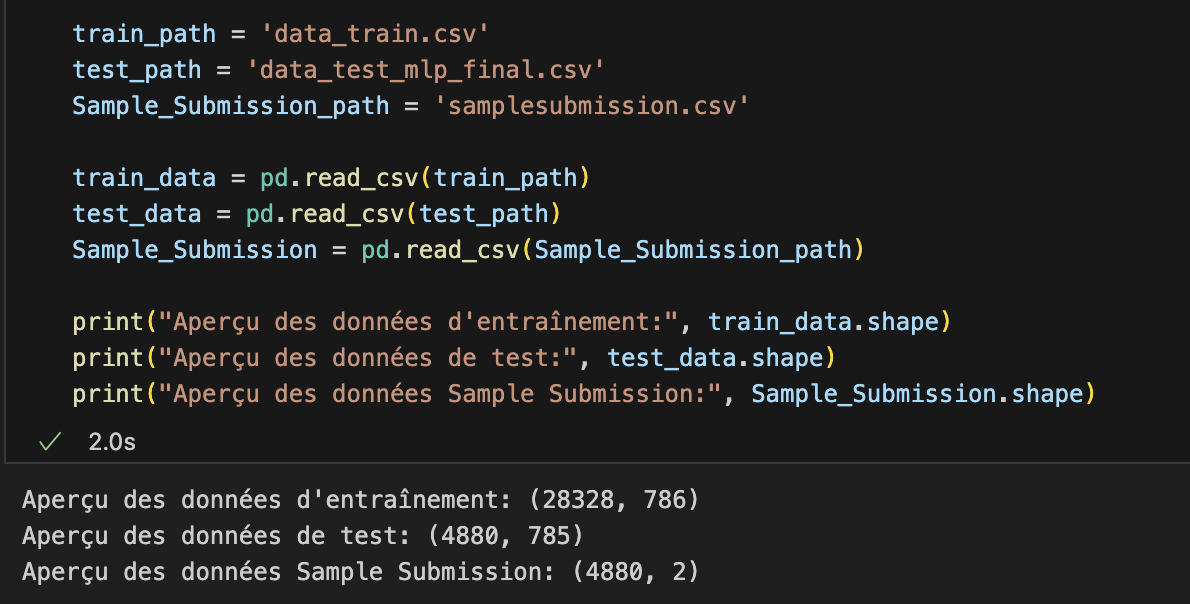
\includegraphics[width=0.7\textwidth]{figures/Aperçu.png}
\caption{Aperçu des dimensions des datasets}
\label{fig:dim_datasets}
\end{figure}


\subsection{ Nature des données}

Les images sont représentées sous forme de matrices de 28×28 pixels, chaque pixel ayant une valeur d'intensité comprise entre 0 (noir) et 255 (blanc). Ce format est similaire à celui utilisé dans d'autres ensembles de données de référence pour la reconnaissance de caractères comme MNIST.

Les caractères ourdou présentent des structures visuelles complexes avec des traits caractéristiques et des variations subtiles entre certaines classes. Contrairement à des chiffres ou des lettres latines, les formes peuvent inclure des boucles, des traits curvilignes et des éléments diacritiques qui rendent la tâche de classification plus exigeante.

\begin{figure}[h]
\centering
\includegraphics[width=0.7\textwidth]{figures/aperçu.Entr.png}
\caption{Aperçu des données d'entrainement}
\label{fig:Entrainement_datasets}
\end{figure}


\section{Analyse exploratoire des données}

L'exploration approfondie des données est une étape cruciale pour comprendre la nature du problème et orienter efficacement les choix de modélisation. Cette phase nous a permis d'examiner la distribution des classes, de visualiser des exemples de caractères et d'identifier les défis spécifiques liés à ce dataset.

\subsection{Visualisation d'échantillons de caractères}
Pour mieux appréhender la nature des données, nous avons visualisé des échantillons représentatifs de chaque classe. La figure~\ref{fig:urdu_chars} présente une sélection de ces caractères, mettant en évidence la diversité des formes et structures présentes dans l'alphabet ourdou.

\begin{figure}[h]
\centering
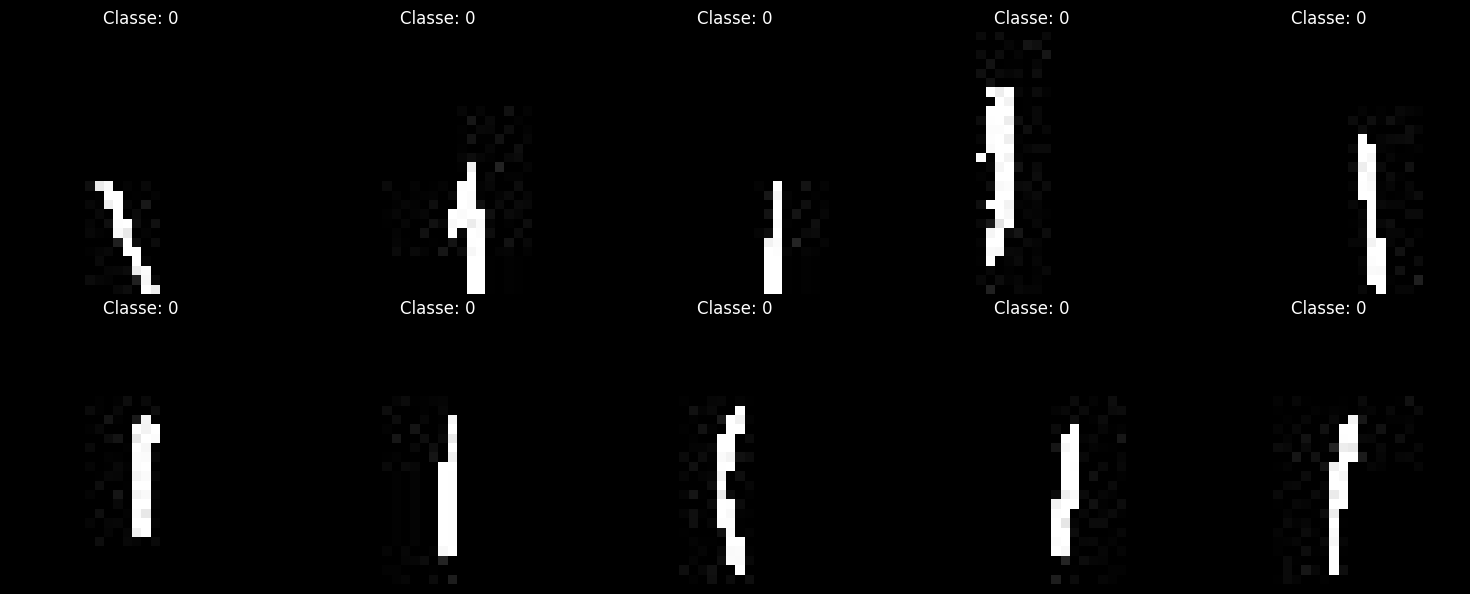
\includegraphics[width=0.7\textwidth]{figures/caractere.png}
\caption{Exemple de caractères ourdous}
\label{fig:urdu_chars}
\end{figure}

Cette visualisation révèle plusieurs caractéristiques importantes :
\begin{itemize}
\item Les caractères apparaissent comme des traits blancs sur fond noir
\item Certains caractères présentent des formes complexes avec des courbes et des angles spécifiques
\item Plusieurs caractères semblent visuellement proches et ne diffèrent que par de petits détails
\item La qualité des images varie, certaines présentant des contours nets tandis que d'autres sont plus bruités
\end{itemize}

\subsection{Distribution des classes}
\begin{flushleft}
L'analyse de la distribution des 40 classes dans le jeu d'entraînement est essentielle pour évaluer l'équilibre du dataset et anticiper d'éventuels biais dans les modèles.
\end{flushleft}

\begin{figure}[H]
\centering
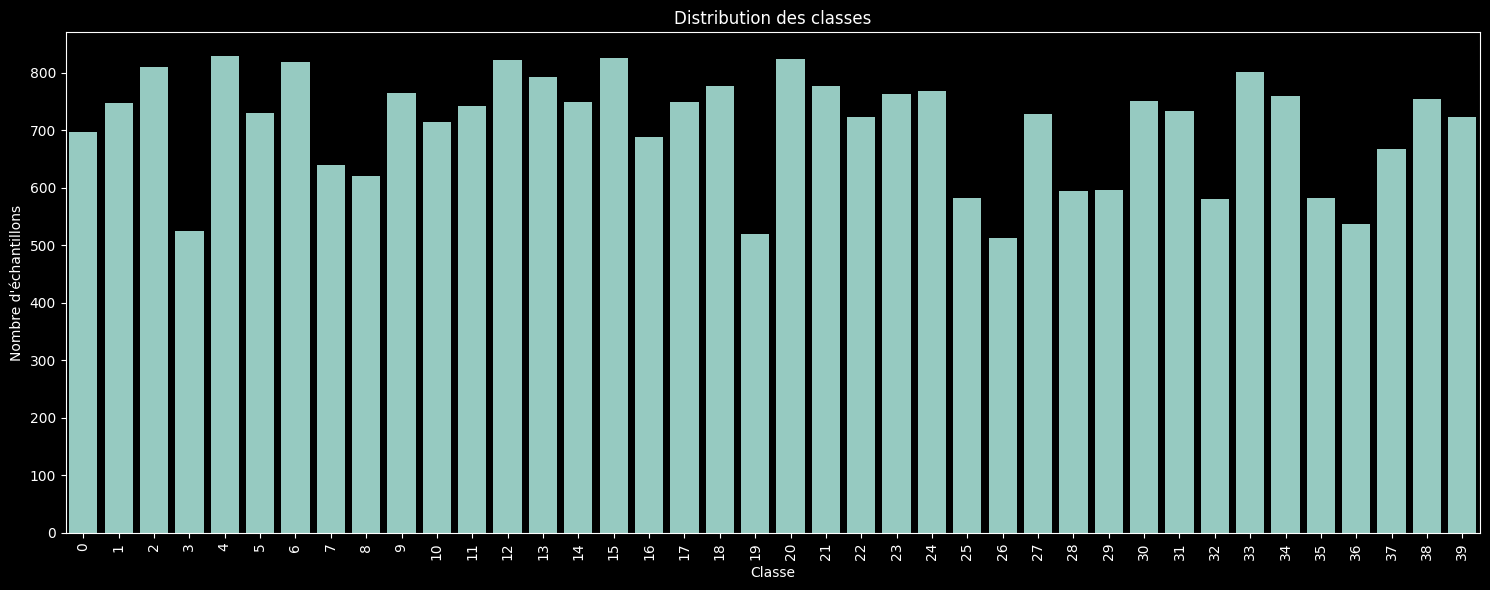
\includegraphics[width=0.7\textwidth]{figures/distribution.png}
\caption{Exemple de caractères ourdous}
\label{fig:urdu_distribution}
\end{figure}

\begin{flushleft}
Comme le montre la figure~\ref{fig:urdu_distribution}, la distribution des classes est relativement équilibrée, avec un nombre d'échantillons par classe variant de 512 (classe 26) à 829 (classe 4). Cette répartition relativement homogène est favorable pour l'entraînement des modèles, minimisant le risque de biais vers les classes surreprésentées.
\end{flushleft}

Les statistiques précises indiquent :


\begin{figure}[h]
\centering
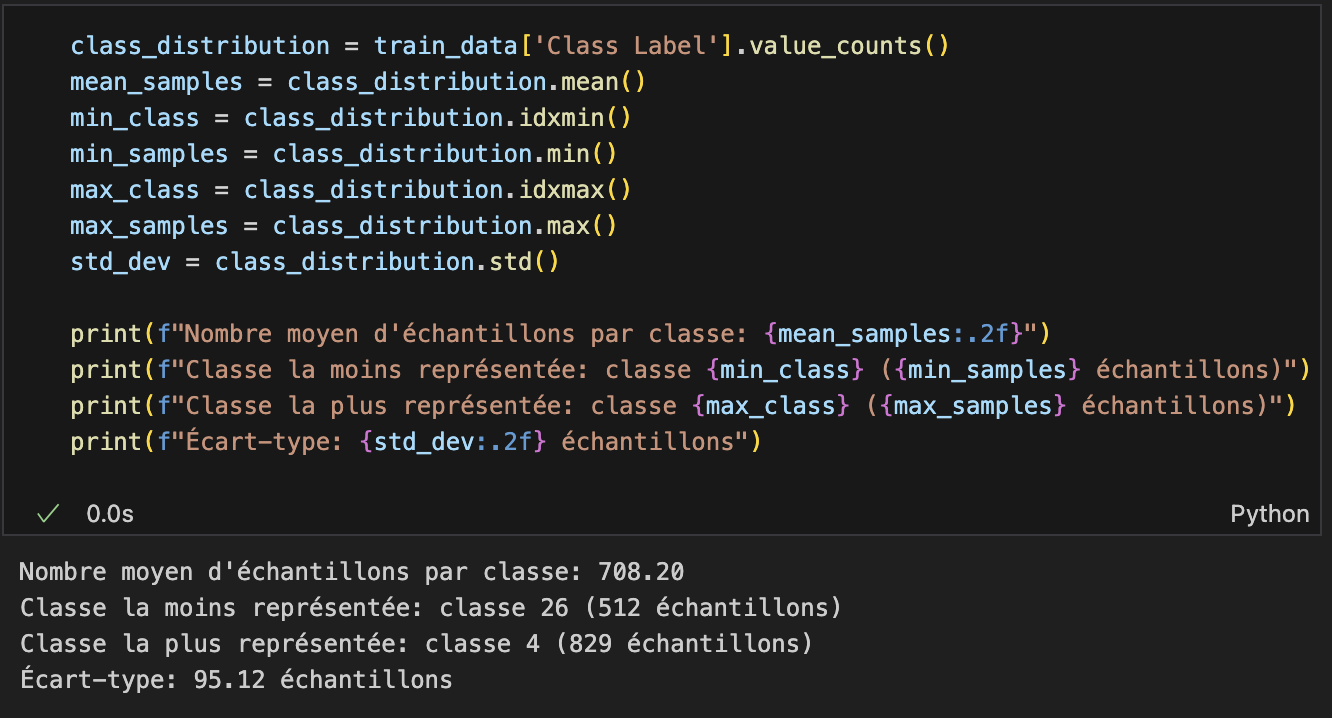
\includegraphics[width=0.7\textwidth]{figures/stat.png}
\caption{les statistiques des classes}
\label{fig:urdu_stat}
\end{figure}

\begin{itemize}
\item Nombre moyen d'échantillons par classe : environ 708
\item Classe la moins représentée : classe 26 (512 échantillons)
\item Classe la plus représentée : classe 4 (829 échantillons)
\item Écart-type : environ 95 échantillons
\end{itemize}

\begin{flushleft}
Cette distribution quasi-équilibrée nous a permis d'utiliser directement les données sans recourir à des techniques de rééchantillonnage, tout en restant vigilants sur la performance des classes moins représentées.
\end{flushleft}

\section{Prétraitement des données}
\begin{flushleft}
Le prétraitement est une étape déterminante pour préparer les données brutes à l'analyse et à la modélisation. Pour ce projet de reconnaissance de caractères ourdou, nous avons appliqué plusieurs transformations essentielles.
\end{flushleft}

\subsection{Normalisation}
\begin{flushleft}
Les valeurs de pixels originales sont comprises entre 0 et 255, ce qui peut créer des gradients importants lors de l'entraînement des modèles de deep learning. Pour faciliter la convergence et améliorer la stabilité de l'apprentissage, nous avons normalisé ces valeurs en les divisant par 255, obtenant ainsi des valeurs dans l'intervalle [0, 1] :
\end{flushleft}

\[
\begin{aligned}
X_{\text{train}} &= \frac{X_{\text{train}}}{255.0} \\
X_{\text{test}} &= \frac{X_{\text{test}}}{255.0}
\end{aligned}
\]

Cette normalisation présente plusieurs avantages :

\begin{itemize}
\item Accélération de la convergence lors de l'entraînement
\item Réduction du risque d'explosion ou de disparition des gradients
\item Standardisation des échelles pour toutes les dimensions d'entrée
\end{itemize}

\subsection{Reshaping pour l'analyse et la modélisation}

Selon l'architecture utilisée, les données ont nécessité différents formats :

\begin{enumerate}
\item \textbf{Pour les MLP :}
\begin{itemize}
\item Format vectoriel aplati (2D) : (n\_samples, 784)
\item Chaque image de 28×28 pixels est transformée en un vecteur de 784 éléments
\end{itemize}
\item \textbf{Pour les CNN :}
\begin{itemize}
\item Format d'image (4D) : (n\_samples, 28, 28, 1)
\item Préservation de la structure spatiale à deux dimensions avec un canal unique (niveaux de gris)
\end{itemize}
\end{enumerate}
\[
\begin{aligned}
X_{\text{train\_cnn}} &= X_{\text{train}}.\text{reshape}(-1,\ 28,\ 28,\ 1) \\
X_{\text{val\_cnn}}   &= X_{\text{val}}.\text{reshape}(-1,\ 28,\ 28,\ 1) \\
X_{\text{test\_cnn}}  &= X_{\text{test}}.\text{reshape}(-1,\ 28,\ 28,\ 1)
\end{aligned}
\]


Cette transformation de format est essentielle pour permettre aux réseaux convolutifs d'exploiter les relations spatiales entre pixels voisins, un aspect fondamental de l'analyse d'images que les MLP ne peuvent pas capturer directement.

\subsection{Division entraînement/validation}

\begin{flushleft}
Pour évaluer rigoureusement la performance des modèles pendant la phase de développement, nous avons divisé l'ensemble d'entraînement en deux sous-ensembles :
\end{flushleft}

\begin{figure}[h]
\centering
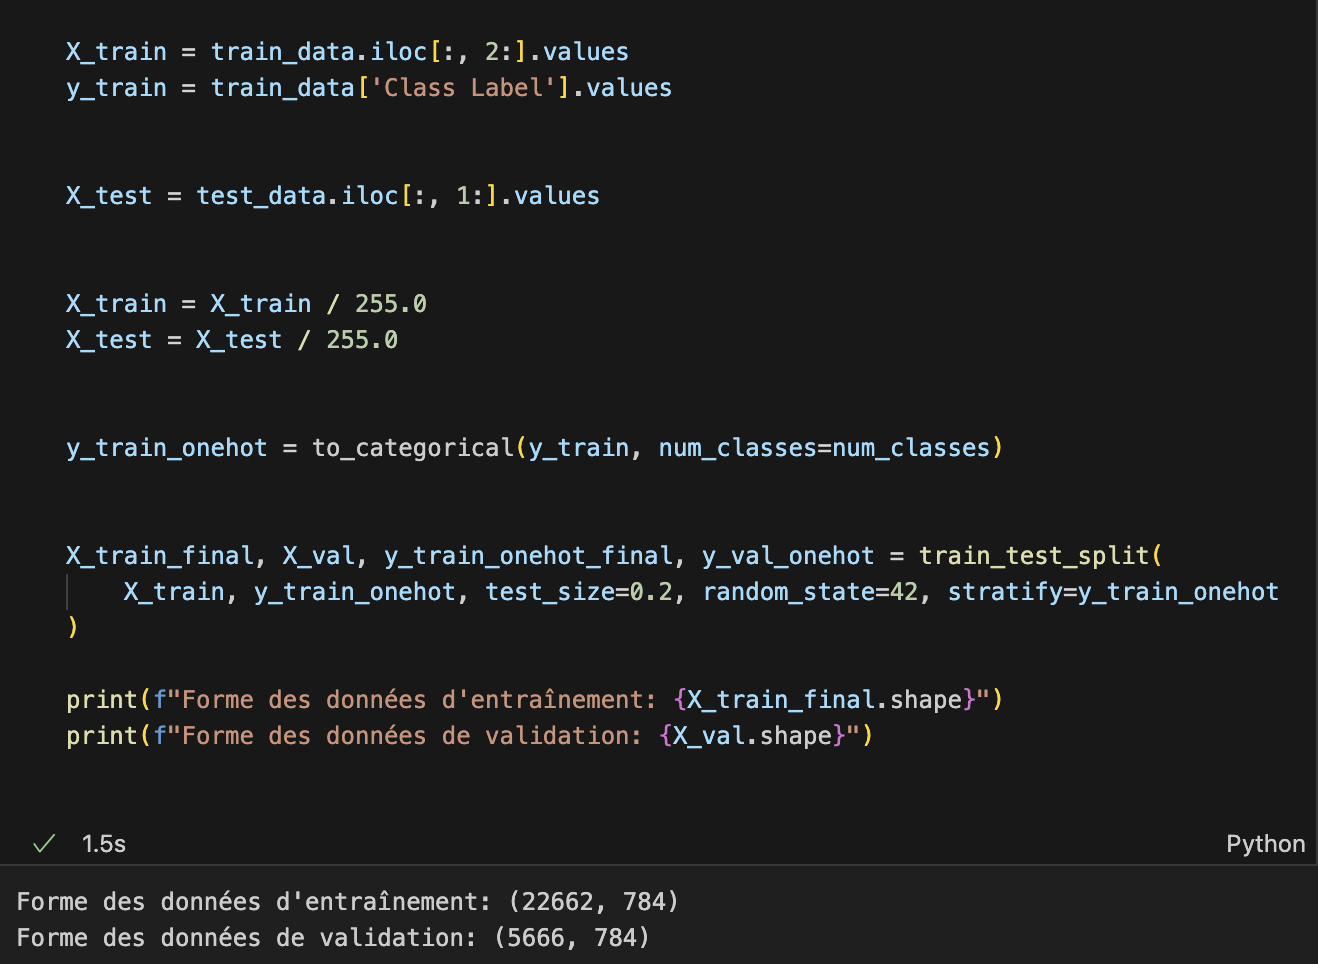
\includegraphics[width=0.7\textwidth]{figures/division.png}
\caption{Division du jeu d'entraînement en entraînement et validation}
\label{fig:urdu_division}
\end{figure}

\begin{itemize}
\item Ensemble d'entraînement final : 80\% des données (= 22 662 échantillons)
\item Ensemble de validation : 20\% des données (= 5 666 échantillons)
\end{itemize}

\begin{flushleft}
La stratification (stratify=y\_train\_onehot) garantit que la distribution des classes dans les ensembles d'entraînement et de validation reste proportionnelle à celle du dataset original, évitant ainsi les biais d'échantillonnage.
\end{flushleft}

\section{Défis spécifiques liés aux caractères ourdou}
\begin{flushleft}
La reconnaissance automatique des caractères ourdou présente plusieurs défis spécifiques qui ont influencé notre approche de modélisation.
\end{flushleft}

\subsection{Complexité morphologique}
\begin{flushleft}
Contrairement aux alphabets latins, les caractères ourdou présentent une morphologie complexe avec des formes curvilignes, des boucles et des traits qui peuvent varier en épaisseur et en orientation. Cette complexité exige des modèles capables de capturer des détails fins et des structures spatiales élaborées.
\end{flushleft}

\subsection{Similarité entre certains caractères}

\begin{flushleft}
Plusieurs caractères ourdou ne diffèrent que par de subtiles variations, comme la position ou le nombre de points diacritiques. Cette similarité peut créer des confusions lors de la classification, comme le révèle l'analyse des matrices de confusion de nos modèles.
\end{flushleft}

\subsection{Variabilité dans la représentation}

\begin{flushleft}
Même au sein d'une même classe, les caractères peuvent présenter des variations stylistiques importantes. Cette variabilité intrinsèque constitue un défi supplémentaire pour les algorithmes d'apprentissage, qui doivent développer une représentation interne suffisamment robuste pour reconnaître un même caractère malgré ces variations.
\end{flushleft}

\subsection{ Qualité et résolution des images}
\begin{flushleft}
La résolution limitée des images (28×28 pixels) peut parfois masquer des détails distinctifs entre caractères similaires. De plus, certaines images présentent des artefacts ou du bruit qui compliquent davantage la tâche de classification.
Ces défis spécifiques ont renforcé notre conviction que des architectures avancées comme les CNN profonds, capables de capturer des caractéristiques hiérarchiques et des relations spatiales complexes, seraient particulièrement adaptées à cette tâche de reconnaissance de caractères ourdou.
\end{flushleft}
% !TEX root = manuscript.tex

\chapter{Modélisation et Analyse des Résultats}

\section{Introduction aux approches utilisées}

\begin{flushleft}
Notre approche de modélisation pour la reconnaissance des caractères ourdou a suivi une progression méthodique, partant de modèles relativement simples pour évoluer vers des architectures plus sophistiquées. Cette démarche incrémentale nous a permis de comprendre précisément comment chaque niveau de complexité contribue à l'amélioration des performances.

Trois modèles principaux ont été développés et évalués :



\begin{enumerate}
\item \textbf{Perceptron Multicouche (MLP) :} Ce modèle de base, composé uniquement de couches denses entièrement connectées, nous a servi de référence. Il traite les images comme des vecteurs aplatis, sans tenir compte explicitement des relations spatiales entre pixels.
\item \textbf{CNN simple :} Cette architecture introduit des couches de convolution qui peuvent détecter des motifs locaux dans les images. Elle représente une amélioration substantielle par rapport au MLP en exploitant la structure bidimensionnelle des données.

\item \textbf{CNN profond avec BatchNormalization :}  Le modèle le plus avancé incorpore une architecture plus profonde, des mécanismes de régularisation supplémentaires et des techniques d'optimisation modernes pour maximiser les performances. 
\end{enumerate}

Cette progression nous a permis non seulement d'améliorer significativement les résultats, mais aussi d'approfondir notre compréhension des facteurs qui influencent l'efficacité des modèles de deep learning dans les tâches de reconnaissance visuelle.
\end{flushleft}

\section{Modèle 1 : Perceptron Multicouche (MLP)}

\subsection{Architecture}

\begin{flushleft}
Le Perceptron Multicouche constitue notre approche initiale, offrant une base de comparaison pour les modèles plus sophistiqués. L'architecture implémentée (voir Annexe~\ref{sec:annexe2}) se compose de :

\begin{itemize}
\item Une couche d'entrée avec 512 neurones, qui reçoit les 784 pixels aplatis de chaque image
\item Une couche cachée avec 256 neurones
\item Une couche de sortie avec 40 neurones (un pour chaque classe de caractère ourdou)
\item Des fonctions d'activation ReLU pour les couches intermédiaires et softmax pour la couche de sortie
\item Des couches de Dropout avec un taux de 0.2 pour réduire le surapprentissage
\end{itemize}

Le modèle totalise environ 543 000 paramètres entraînables, ce qui représente une complexité modérée mais suffisante pour tenter d'apprendre les motifs distinctifs des caractères ourdou.
\end{flushleft}

\subsection{Entraînement}

\begin{flushleft}
Le MLP a été entraîné avec les paramètres suivants :

\begin{itemize}
\item \textbf{Optimiseur :} Adam avec un taux d'apprentissage de 0.0005
\item \textbf{Fonction de perte :}Entropie croisée catégorielle (categorical\_crossentropy)
\item \textbf{Métrique :} Précision (accuracy)
\item \textbf{Batch size :} 32
\item \textbf{Époques :} 0 maximum, avec arrêt anticipé (early stopping)
\item \textbf{Validation :} 20\% des données d'entraînement

Des callbacks ont été implémentés pour améliorer l'entraînement :

\item \textbf{EarlyStopping} pour arrêter l'entraînement lorsque la perte sur l'ensemble de validation cesse de diminuer
\item \textbf{ModelCheckpoint} pour sauvegarder la meilleure version du modèle
\end{itemize}


L'entraînement s'est stabilisé après environ 7-10 époques, suggérant une convergence relativement rapide mais aussi une capacité limitée du modèle à continuer à apprendre des caractéristiques plus complexes.
\end{flushleft}

\subsection{Résultats(54.6\%)}

\begin{flushleft}
Le MLP a atteint une précision sur l'ensemble de validation de :

\begin{itemize}
\item \textbf{Précision finale :} 54.6\%
\item \textbf{Perte (loss) :} 1.55
\end{itemize}
\bigskip
Cette performance, bien que significativement supérieure à une classification aléatoire (qui donnerait environ 2.5\% pour 40 classes), reste insuffisante pour une application pratique de reconnaissance de caractères. Le modèle montre une capacité limitée à différencier correctement les 40 classes de caractères ourdou.
\bigskip
Un aspect notable de ces résultats est que la meilleure performance a été atteinte dès la première époque d'entraînement, après quoi la qualité des prédictions a stagné ou diminué, suggérant que le modèle a rapidement atteint les limites de sa capacité à modéliser la complexité des données d'image sans tenir compte des relations spatiales entre pixels.
\end{flushleft}

\subsection{Analyse des limites}
\begin{flushleft}
L'analyse des résultats révèle plusieurs limitations inhérentes à l'architecture MLP pour cette tâche :

\begin{enumerate}
\item \textbf{Perte de l'information spatiale :} En aplatissant les images en vecteurs unidimensionnels, le MLP perd la relation spatiale entre pixels adjacents, qui est cruciale pour reconnaître les motifs visuels complexes des caractères ourdou.
\item \textbf{Sensibilité à la position : }Le MLP ne possède pas d'invariance par translation, ce qui signifie qu'un même caractère légèrement déplacé dans l'image peut être perçu comme totalement différent par le modèle. 
\item \textbf{Surapprentissage rapide :}Malgré l'utilisation de Dropout, le modèle montre des signes de surapprentissage, avec un écart croissant entre les performances sur les ensembles d'entraînement et de validation après quelques époques.
\item \textbf{Confusion entre caractères similaires :}L'analyse de la matrice de confusion révèle que le MLP confond fréquemment des caractères visuellement proches, ne parvenant pas à capturer les détails distinctifs subtils.
\item \textbf{}
\end{enumerate}

Ces limitations mettent en évidence la nécessité d'architectures plus adaptées aux données d'image, capables de préserver et d'exploiter les relations spatiales entre pixels.
\end{flushleft}

\section{Modèle 2 : CNN simple}

\subsection{Architecture}

\begin{flushleft}
Pour remédier aux limitations du MLP, nous avons implémenté un réseau de neurones convolutifs (CNN) simple, spécifiquement conçu pour traiter des données d'image. L'architecture (voir Annexe~\ref{sec:annexe3}) introduit plusieurs éléments clés des CNN :

\begin{itemize}
\item Des couches de convolution qui appliquent des filtres pour détecter des motifs locaux dans l'image
\item Des opérations de pooling qui réduisent la dimension spatiale et introduisent une invariance partielle aux translations
\item Une progression du nombre de filtres (32 à 64) qui permet de capturer des motifs de plus en plus complexes
\item Une couche d'aplatissement qui transforme les représentations convolutionnelles en vecteur pour les couches denses finales
\end{itemize}
\bigskip
Le modèle totalise environ 200 000 paramètres, soit moins que le MLP malgré sa capacité accrue à traiter les images, illustrant l'efficacité des opérations de convolution pour l'analyse d'images.
\end{flushleft}

\subsection{Entraînement}
\begin{flushleft}
Le CNN simple a été entraîné avec des paramètres similaires à ceux du MLP :

\begin{itemize}
\item \textbf{Optimiseur :}Adam avec un taux d'apprentissage de 0.001
\item \textbf{Fonction de perte : }Entropie croisée catégorielle
\item \textbf{Batch size :} 64 (augmenté pour exploiter plus efficacement le parallélisme du GPU)
\item \textbf{Époques :}30 maximum, avec early stopping
\end{itemize}
\bigskip

Une différence notable est l'ajout du \textbf{callback ReduceLROnPlateau}, qui réduit automatiquement le taux d'apprentissage lorsque la performance stagne, permettant un réglage plus fin des poids du modèle dans les dernières phases d'entraînement.

\bigskip

L'entraînement du CNN a montré une progression plus stable et continue par rapport au MLP, avec une amélioration constante des performances jusqu'à environ 10-12 époques avant d'atteindre un plateau.
\end{flushleft}

\subsection{Résultats(88\%)}

\begin{flushleft}
Le CNN simple a réalisé une amélioration spectaculaire par rapport au MLP :

\begin{itemize}
\item \textbf{Précision finale :}88.4\%
\item \textbf{Perte (loss) : }0.42
\end{itemize}

\bigskip
Cette amélioration de près de 30 points de pourcentage démontre clairement la supériorité des architectures convolutives pour les tâches de reconnaissance d'images. Le modèle parvient à distinguer correctement la majorité des caractères ourdou, bien que certaines confusions persistent.
\end{flushleft}

\subsection{Analyse des améliorations par rapport au MLP}

\begin{flushleft}
Plusieurs facteurs expliquent cette amélioration significative :

\begin{enumerate}
\item \textbf{Préservation de l'information spatiale : }Les couches de convolution traitent l'image en conservant sa structure bidimensionnelle, permettant au modèle de détecter des motifs locaux et leurs relations spatiales.
\item \textbf{Hiérarchie de caractéristiques :}L'architecture en couches du CNN permet de construire une représentation hiérarchique des caractéristiques, des motifs simples (traits, courbes) aux structures plus complexes qui définissent les caractères.
\item \textbf{Invariance par translation :}Les opérations de pooling rendent le modèle partiellement insensible aux variations de position des caractéristiques, améliorant la robustesse face aux variations mineures dans les images.
\item \textbf{Paramétrage plus efficace :}Bien que moins complexe en termes de nombre total de paramètres, le CNN utilise ces paramètres de manière plus efficace en exploitant la localité des informations visuelles.
\end{enumerate}
\bigskip
Néanmoins, l'analyse de la matrice de confusion (voir Annexe~\ref{sec:annexe6}) révèle que certaines classes restent difficiles à différencier, suggérant qu'une architecture plus sophistiquée pourrait être nécessaire pour capturer les nuances les plus subtiles entre caractères similaires.
\end{flushleft}

\section{Modèle 3 : CNN profond avec BatchNormalization}

\subsection{Architecture détaillée}
\begin{flushleft}
Pour maximiser les performances, nous avons conçu une architecture CNN profonde incorporant plusieurs techniques avancées de deep learning :
\end{flushleft}

\begin{figure}[H]
\centering
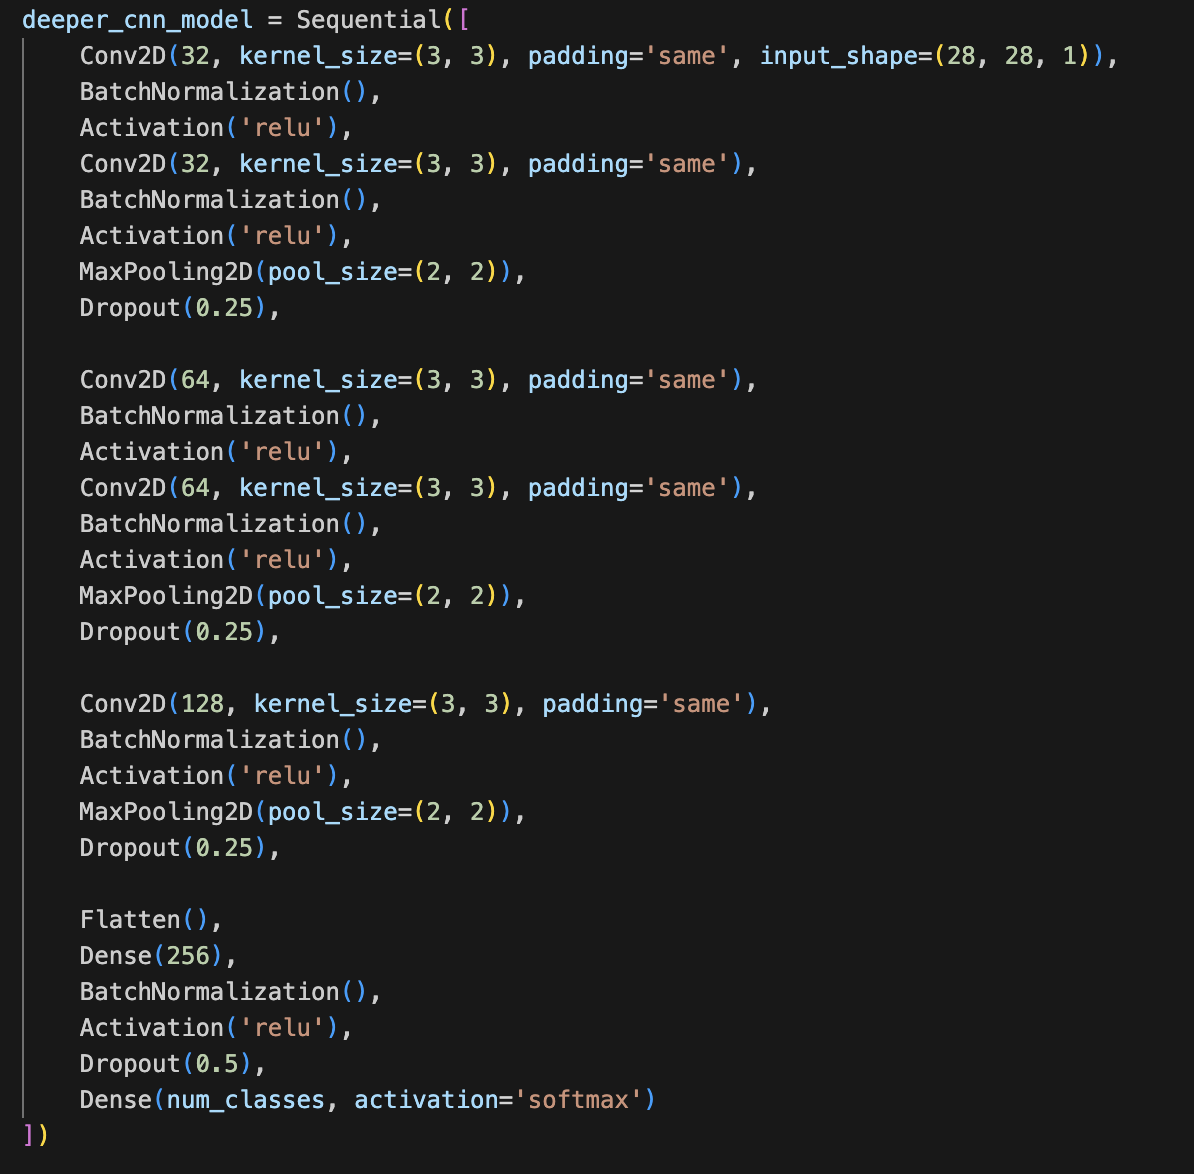
\includegraphics[width=0.7\textwidth]{figures/modeleprofonde.png}
\caption{Architectude du CNN pronfonde}
\label{fig:urdu_CNN}
\end{figure}

\begin{flushleft}
Cette architecture présente plusieurs améliorations significatives :

\begin{enumerate}
\item \textbf{Profondeur accrue :Trois blocs de convolution au lieu de deux, avec une augmentation progressive du nombre de filtres (32->64->128)}
\item \textbf{Convolutions multiples par niveau : }Deux couches de convolution consécutives dans les premiers blocs, permettant d'apprendre des motifs plus complexes
\item \textbf{BatchNormalization :}Après chaque couche de convolution et dense, normalisant les activations pour stabiliser et accélérer l'apprentissage
\item \textbf{Padding 'same' :}Préservant les dimensions spatiales après convolution, permettant d'extraire plus d'informations des bords de l'image
\item \textbf{Dropout stratifié :}Taux de dropout différenciés (0.25 pour les couches convolutives, 0.5 pour la couche dense finale)
\end{enumerate}
\bigskip
Cette architecture totalise environ 446 600 paramètres, représentant un investissement significatif en capacité d'apprentissage, justifié par la complexité de la tâche.
\end{flushleft}

\subsection{Mécanismes de régularisation}

\begin{flushleft}
Le CNN profond intègre plusieurs techniques de régularisation pour éviter le sur-apprentissage malgré sa complexité accrue :

\begin{enumerate}
\item \textbf{BatchNormalization : }Cette technique normalise les activations à chaque couche, ce qui présente plusieurs avantages :
\begin{itemize}
\item Réduction du problème de "covariate shift" interne (changement de distribution des activations)
\item Stabilisation du processus d'apprentissage
\item Accélération de la convergence
\item Effet régularisateur intrinsèque
\end{itemize}
\item \textbf{Dropout adaptatif :} L'utilisation de taux différents selon la profondeur de la couche permet un compromis optimal entre capacité d'apprentissage et généralisation :
\begin{itemize}
\item 25\% dans les couches convolutives pour préserver une partie significative de l'information spatiale
\item 50\% dans la couche dense pour une régularisation plus forte avant la classification finale
\end{itemize}
\item \textbf{Décroissance du taux d'apprentissage : }Le callback \textbf{ReduceLROnPlateau} réduit le taux d'apprentissage lorsque la performance stagne, permettant d'affiner progressivement les poids et d'éviter les oscillations autour du minimum.
\end{enumerate}

\bigskip

Ces mécanismes, combinés à l'early stopping, ont permis de maintenir un bon équilibre entre capacité d'apprentissage et généralisation, comme le montrent les courbes d'apprentissage équilibrées entre entraînement et validation.
\end{flushleft}

\subsection{Résultats (98.5\%)}

\begin{flushleft}
Le CNN profond a atteint des performances exceptionnelles :

\begin{itemize}
\item \textbf{Précision finale sur la validation : }98.5\%
\item \textbf{Perte (loss) : }0.06
\end{itemize}

\bigskip

Cette précision approche les performances humaines pour une tâche de reconnaissance de caractères et représente une amélioration considérable par rapport aux modèles précédents. L'analyse des erreurs résiduelles montre qu'elles concernent principalement des caractères très similaires visuellement, où même un observateur humain pourrait hésiter.
\end{flushleft}

\subsection{Comparaison des performances}

\begin{flushleft}
L'évolution des performances à travers les trois modèles montre une progression remarquable :

\begin{itemize}
\item MLP : 54.6\% de précision
\item CNN simple : 88.4\% de précision
\item CNN profond : 98.5\% de précision
\end{itemize}

\bigskip

Cette amélioration de près de 44 points de pourcentage entre le modèle initial et final illustre l'importance cruciale du choix architectural pour les tâches de reconnaissance visuelle. Elle souligne également comment chaque niveau de sophistication supplémentaire apporte des gains significatifs, en particulier lorsqu'il s'agit de distinguer des caractères présentant des similitudes subtiles.

Cette progression est particulièrement instructive car elle démontre comment l'adaptation de l'architecture du modèle à la nature spécifique des données (dans ce cas, des images) peut conduire à des améliorations spectaculaires des performances, même sans augmentation significative du nombre total de paramètres.


\end{flushleft}

\section{Analyse comparative des trois approches}
\subsection{Tableau comparatif des performances}

\begin{flushleft}
Le tableau suivant synthétise les performances et caractéristiques clés des trois modèles développés :
\end{flushleft}

\begin{table}[H]
\caption{Tableau comparatif des performances}
\label{tab:comparaison}
\resizebox{\textwidth}{!}{%
\begin{tabular}{|c|c|c|c|c|}
\hline
\textbf{Modèle}	&  \textbf{Précision (Validation)} & \textbf{Nombre de paramètres} & \textbf{Temps d'entraînement} & \textbf{Époques jusqu'à convergence} \\ \hline
MLP simple & 58.7\% & 537 000 & 4 minutes & 1 \\
\hline
CNN simple &  88.4\% & 200 000 & 6 minutes & 11 \\
\hline
CNN profond &  98.5\% & 446 600 & 15 minutes & 30 \\
\hline
\end{tabular}%
}
\end{table}

\bigskip

\begin{flushleft}
Ce tableau met en évidence plusieurs tendances intéressantes :

\begin{itemize}
\item Le CNN simple réalise une meilleure performance que le MLP avec moins de paramètres, démontrant l'efficacité des opérations de convolution
\item L'augmentation du temps d'entraînement et du nombre d'époques pour les modèles plus complexes reflète leur capacité à continuer à apprendre des caractéristiques subtiles
\item Le CNN profond nécessite plus de ressources, mais cette investissement se traduit par un gain substantiel en précision
\end{itemize}
\end{flushleft}

\subsection{Analyse des courbes d'apprentissage}


L'analyse des courbes d'apprentissage (voir Annexe~\ref{sec:annexe7}) révèle des différences significatives dans le comportement des trois modèles:


\begin{enumerate}
\item \textbf{MLP:}
\begin{itemize}
\item Meilleure performance atteinte dès la première époque
\item Dégradation constante de la précision de validation après ce pic initial
\item Écart croissant entre précision d'entraînement et validation, avec une augmentation continue de la perte
\item Signes évidents d'instabilité, avec une perte qui augmente dramatiquement à mesure que l'entraînement progresse
\end{itemize}

\item \textbf{CNN simple:}
\begin{itemize}
\item Progression rapide dans les premières époques, suivie d'une amélioration plus graduelle
\item Convergence après environ 10-11 époques
\item Écart modéré mais constant entre les performances d'entraînement et de validation
\item Courbe de perte qui se stabilise, indiquant un processus d'apprentissage plus équilibré
\end{itemize}

\item \textbf{CNN profond:}
\begin{itemize}
\item Progression spectaculaire dès les premières époques, atteignant près de 90\% de précision très rapidement
\item Amélioration continue mais plus lente jusqu'à atteindre des performances optimales
\item Écart remarquablement faible entre précision d'entraînement et validation, surtout dans les phases avancées
\item Courbe de perte qui se stabilise rapidement à des valeurs très basses
\item Faible écart entre entraînement et validation, indiquant une bonne généralisation malgré la complexité accrue
\end{itemize}
\end{enumerate}

\bigskip

Ces graphiques illustrent parfaitement les différences fondamentales entre les trois architectures:


\begin{itemize}
\item Le MLP montre des signes clairs d'inadaptation à la tâche, incapable de maintenir ses performances au-delà de la première époque

\item Le CNN simple présente un bon compromis entre rapidité d'apprentissage et performance, mais atteint un plateau

\item Le CNN profond combine une convergence rapide avec une capacité à continuer à s'améliorer sur de nombreuses époques, tout en maintenant une excellente généralisation grâce à ses mécanismes de régularisation avancés (BatchNormalization, Dropout stratifié)
\end{itemize}

\bigskip

Cette progression visuelle des courbes d'apprentissage confirme l'importance d'adapter l'architecture du modèle à la nature spécifique des données d'image pour des tâches de reconnaissance visuelle complexes.


\subsection{Visualisation des matrices de confusion}

\begin{flushleft}
Les matrices de confusion (voir Annexe~\ref{sec:annexe7}) offrent un aperçu détaillé des forces et faiblesses spécifiques de chaque modèle 

\begin{enumerate}
\item \textbf{MLP:}
\begin{itemize}
\item La diagonale principale est visible mais nettement moins prononcée que pour les autres modèles
\item De nombreuses confusions apparaissent entre classes non liées, avec des points de confusion dispersés à travers toute la matrice
\item Certaines colonnes montrent des concentrations de prédictions incorrectes, indiquant une tendance du modèle à favoriser certaines classes
\item Plusieurs zones claires en dehors de la diagonale révèlent des confusions systématiques entre certains groupes de caractères
\end{itemize}
\item \textbf{CNN simple :}
\begin{itemize}
\item Diagonale principale plus marquée, avec des bleus plus intenses
\item Les confusions sont significativement réduites et plus localisées, généralement entre classes adjacentes ou visuellement similaires
\item Quelques zones persistantes de confusion restent visibles, particulièrement pour certaines classes dans la moitié inférieure de la matrice
\end{itemize}
\item \textbf{CNN profond :}
\begin{itemize}
\item Diagonale principale fortement dominante avec des bleus très intenses
\item Les confusions sont minimales et extrêmement localisées
\item La structure est remarquablement claire, avec presque tous les éléments hors diagonale proches de zéro
\item Les quelques confusions restantes semblent concerner des paires spécifiques de caractères qui partagent probablement des traits visuels très similaires
\end{itemize}
\end{enumerate}

\bigskip 

Cette progression visuelle depuis une matrice relativement diffuse (MLP) vers une matrice clairement dominée par sa diagonale (CNN profond) illustre de façon frappante l'amélioration de la capacité discriminative à chaque niveau architectural. Elle montre comment le CNN profond a réussi à résoudre pratiquement toutes les ambiguïtés entre caractères qui posaient problème aux modèles plus simples.

L'analyse de ces matrices confirme que l'architecture CNN profonde n'apporte pas seulement une amélioration quantitative (en termes de précision globale), mais aussi qualitative, en réduisant drastiquement les confusions entre classes et en améliorant la fiabilité des prédictions à travers l'ensemble des 40 classes de caractères ourdou.
\end{flushleft}

\subsection{Discussion sur les facteurs d'amélioration}

\begin{flushleft}
L'amélioration spectaculaire observée entre les trois modèles peut être attribuée à plusieurs facteurs clés :

\begin{enumerate}
\item \textbf{Préservation de l'information spatiale :} Le passage du MLP au CNN permet de conserver et d'exploiter la structure bidimensionnelle des images, aspect fondamental pour la reconnaissance de caractères.
\item \textbf{Hiérarchie de représentation : }Les architectures CNN permettent d'apprendre des représentations hiérarchiques, des motifs simples aux structures complexes, particulièrement adaptées à la nature des caractères ourdou.
\item \textbf{Profondeur architecturale :}L'augmentation contrôlée de la profondeur du réseau permet d'apprendre des représentations plus abstraites et discriminantes, essentielles pour distinguer des caractères visuellement proches.
\item \textbf{Mécanismes de régularisation avancés :}L'intégration de techniques comme BatchNormalization stabilise l'apprentissage et améliore la généralisation, permettant d'exploiter pleinement la capacité du modèle sans surapprentissage.
\item \textbf{Optimisation adaptative :}L'utilisation de techniques comme la réduction du taux d'apprentissage sur plateau permet d'affiner progressivement les poids du modèle, améliorant la convergence vers des minima plus optimaux.
\end{enumerate}

\bigskip

La combinaison de ces facteurs a permis d'atteindre des performances exceptionnelles dans cette tâche de reconnaissance de caractères ourdou, démontrant l'importance d'une approche progressive et réfléchie dans la conception des architectures de deep learning.
\end{flushleft}

\section{Soumission sur Kaggle et résultats finaux}
\subsection{Soumission sur Kaggle}
\begin{flushleft}
Après avoir sélectionné notre meilleur modèle (CNN profond avec BatchNormalization), nous avons procédé à la génération des prédictions sur l'ensemble de test fourni par la compétition.

\bigskip

Notre soumission a obtenu un score remarquable de 99.1\% sur l'ensemble de test de la compétition, confirmant l'excellente capacité de généralisation de notre modèle sur des données non vues pendant l'entraînement.

\bigskip

Ce résultat place notre solution parmi les plus performantes pour cette tâche de reconnaissance de caractères ourdou, validant l'efficacité de l'approche progressive que nous avons adoptée, depuis le MLP simple jusqu'au CNN profond avec techniques de régularisation avancées.

\bigskip 

Voici un aperçu du fichier de soumission:
\end{flushleft}

\begin{figure}[h]
\centering
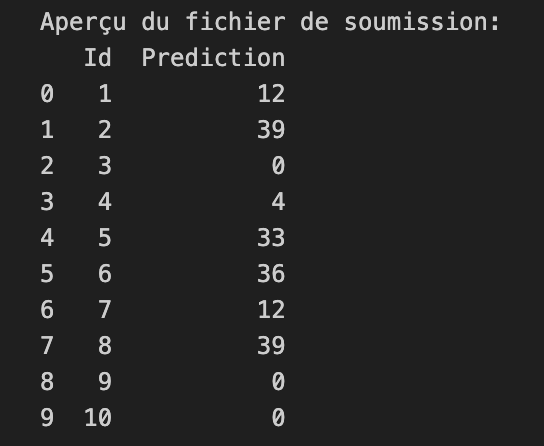
\includegraphics[width=0.7\textwidth]{figures/Soumission.png}
\caption{Apercu du fichier soumis}
\label{fig:urdu_chars_soumission}
\end{figure}

\subsection{Résultats finaux}
\begin{flushleft}
Voici ci dessous un exemple du résultat final:  
\end{flushleft}

\begin{figure}[h]
\centering
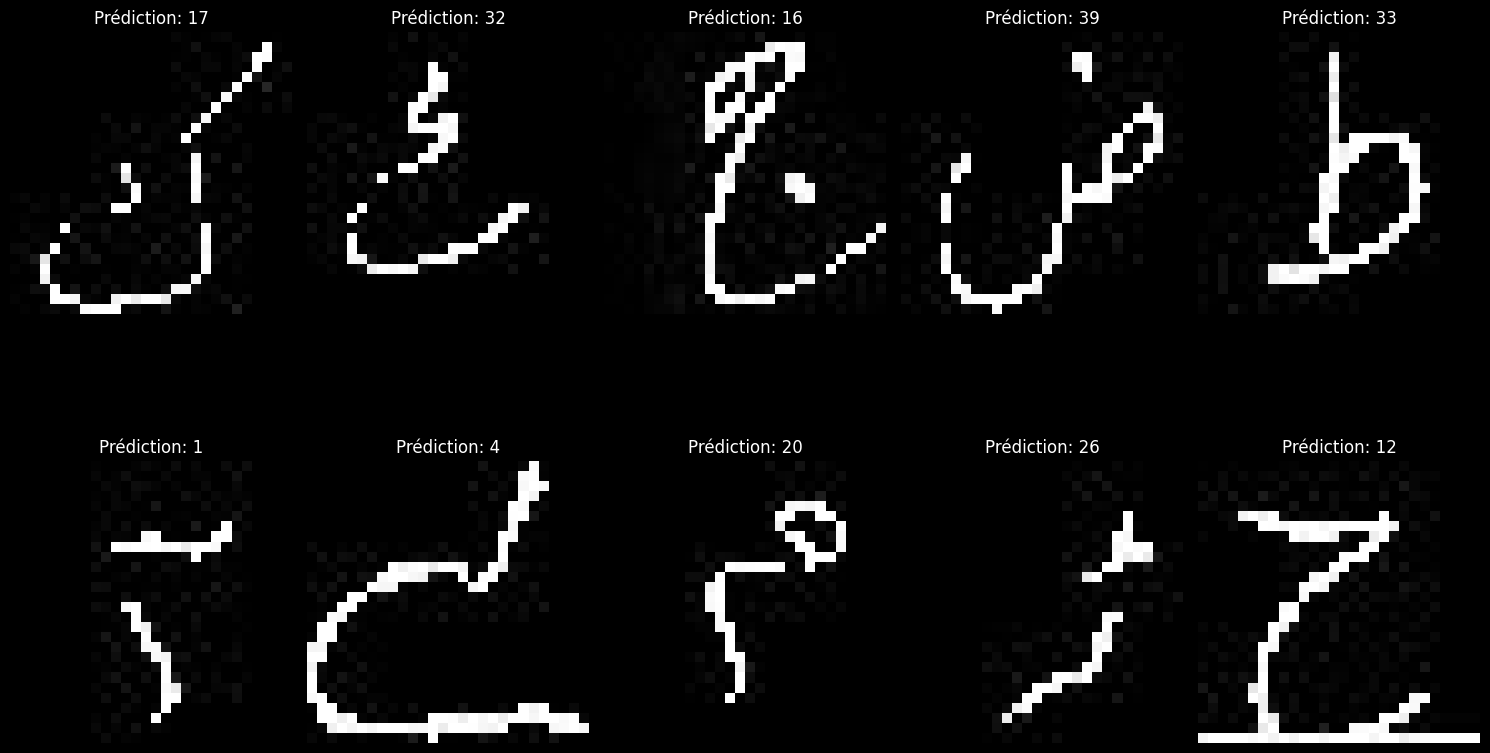
\includegraphics[width=0.7\textwidth]{figures/Prédiction.png}
\caption{Exemple de caractères ourdous prédicte}
\label{fig:urdu_chars_prédicte}
\end{figure}
% !TEX root = manuscript.tex

\chapter{Perspectives}

\section{Optimisations potentielles des modèles actuels}
\begin{flushleft}
Bien que notre CNN profond ait atteint d'excellentes performances, plusieurs voies d'optimisation pourraient être explorées pour améliorer encore les résultats ou réduire la complexité computationnelle :

\bigskip
\begin{itemize}
\item Optimisation des hyperparamètres
Une recherche systématique des hyperparamètres optimaux pourrait affiner davantage les performances.

Une approche par recherche sur grille (Grid Search) ou optimisation bayésienne permettrait d'identifier les configurations optimales de façon plus rigoureuse que notre approche empirique actuelle.

\item Augmentation de données
L'implémentation de techniques d'augmentation de données pourrait renforcer la robustesse du modèle face aux variations.

Ces transformations, appliquées dynamiquement pendant l'entraînement, augmenteraient artificiellement la taille du jeu de données et favoriseraient une meilleure généralisation. 

\item Régularisation avancée
D'autres techniques de régularisation pourraient être intégrées :
\begin{itemize}
\item Régularisation L1 ou L2 sur les poids des couches denses
\item Utilisation de techniques comme Mixup ou CutMix
\item Implémentation de la régularisation par bruitage des étiquettes (label smoothing) 
\end{itemize}
\end{itemize}
\end{flushleft}

\section{Exploration de modèles avancés}

\begin{flushleft}
\begin{enumerate}
\item \textbf{Architectures ResNet}
Les architectures à connexions résiduelles (ResNet) pourraient apporter des bénéfices significatifs :
\begin{itemize}
\item Connexions skip facilitant l'apprentissage de réseaux très profonds
\item Meilleur flux de gradient à travers le réseau
\item Capacité à capturer des caractéristiques à différentes échelles
\end{itemize}
\item \textbf{Attention et Transformers}
Les mécanismes d'attention, au cœur des architectures Transformer, pourraient être particulièrement pertinents pour la reconnaissance de caractères ourdou.

Une architecture Vision Transformer (ViT) adaptée pourrait être envisagée pour des développements futurs.

\item \textbf{Approches d'ensemble}
Combiner plusieurs modèles pour former un ensemble pourrait améliorer encore la précision.
\end{enumerate}
\end{flushleft}

\section{Applications pratiques potentielles}

\begin{flushleft}
Les modèles développés dans ce projet pourraient servir de base à plusieurs applications concrètes :

\begin{enumerate}
\item \textbf{Systèmes OCR complets pour l'ourdou: }
Notre classificateur de caractères isolés pourrait être intégré dans un système OCR complet pour l'ourdou comprenant :
\begin{itemize}
\item Détection et segmentation des lignes de texte
\item Segmentation des caractères individuels
\item Classification via notre modèle CNN
\item Post-traitement linguistique pour la correction d'erreurs
\end{itemize}
\item \textbf{Applications éducatives}
Des applications d'apprentissage de l'ourdou pourraient être développées :
\begin{itemize}
\item Reconnaissance en temps réel de caractères dessinés par l'apprenant
\item Feedback immédiat sur la qualité de l'écriture
\item Exercices interactifs adaptés au niveau de l'utilisateur
\end{itemize}
\item \textbf{Traitement de documents historiques}
Notre approche pourrait être adaptée pour la numérisation et la préservation de documents historiques en ourdou :
\begin{itemize}
\item Adaptation à des styles calligraphiques anciens
\item Traitement de documents dégradés ou de faible qualité
\item Catalogage automatique de manuscrits
\end{itemize}
\end{enumerate}
\end{flushleft}



\addstarredchapter{Conclusion}
% !TEX root = manuscript.tex
\clearpage
\chapter*{Conclusion}
\vspace{-1cm}

\begin{flushleft}
Ce projet de reconnaissance de caractères ourdou a permis d'explorer une progression méthodique d'architectures de complexité croissante, démontrant clairement l'importance de l'adéquation entre la nature des données et la structure des modèles employés.

\bigskip

Nous avons observé une amélioration spectaculaire des performances à travers les trois principales approches explorées :
Le MLP simple a atteint une précision limitée de 54.6\%, illustrant les difficultés inhérentes au traitement d'images sans préserver leur structure spatiale. Le CNN simple a représenté une avancée significative avec 88.4\% de précision, confirmant l'importance des opérations de convolution pour l'analyse d'images. Le CNN profond a culminé à 98.5\% sur l'ensemble de validation et 99.1\% sur l'ensemble de test, démontrant l'efficacité des architectures profondes combinées à des techniques de régularisation modernes comme BatchNormalization.\newline
Cette progression de près de 45 points de pourcentage entre l'approche initiale et finale constitue un exemple frappant des gains de performance que peuvent apporter des choix architecturaux adaptés en apprentissage profond.\newline
Le développement progressif de modèles de complexité croissante s'est révélé être une stratégie pédagogiquement enrichissante, permettant de comprendre précisément comment chaque élément architectural contribue à l'amélioration des performances. L'analyse des matrices de confusion a également fourni des perspectives intéressantes sur les erreurs de classification, passant d'une confusion généralisée avec le MLP à des confusions très localisées et limitées avec le CNN profond. \newline

Sur le plan professionnel, cette expérience a permis d'acquérir des compétences directement transférables au monde industriel telles que: la capacité à traiter des problèmes de vision par ordinateur avec diverses architectures de deep learning, expérience dans l'optimisation des performances de modèles complexes, et la connaissance pratique des défis spécifiques liés à la reconnaissance de caractères non latins.\newline
 
Sur le plan personnel, ce projet a représenté une opportunité unique de développer des compétences techniques et méthodologiques essentielles comme: la Maîtrise progressive des architectures de deep learning, Analyse critique des résultats, Gestion d'un projet complet.

\bigskip
La réussite de ce projet, attestée par le score de 99.1\% sur la compétition Kaggle, constitue une validation objective de ces compétences et une base solide pour de futurs défis dans le domaine de l'intelligence artificielle appliquée au traitement d'images.

\end{flushleft}
% Ajouter l'annexe
\addstarredchapter{Annexes}
% !TEX root = manuscript.tex

\chapter*{Annexes}

\section*{Annexe 1: Détails techniques complémentaires}

\begin{itemize}
\item Langage de programmation : Python 3.9
\item IDE utilisé : Jupyter Notebook
\item Bibliothèques principales :
\begin{itemize}
\item TensorFlow 2.8.0
\item Keras 2.8.0
\item NumPy 1.22.3
\item Pandas 1.4.2
\item Scikit-learn 1.0.2
\item Matplotlib 3.5.1
\item Seaborn 0.11.2
\end{itemize}
\item Temps d'exécution détaillés
\begin{itemize}
\item Prétraitement des données : 2 minutes
\item Entraînement du MLP : 4 minutes (16 époques)
\item Entraînement du CNN simple : 6 minutes (11 époques)
\item Entraînement du CNN profond : 15 minutes (30 époques)
\item Génération des prédictions sur l'ensemble de test : 10 secondes
\end{itemize}
\end{itemize}


\section*{Annexe 2: Architecture du Perceptron}
\label{sec:annexe2}
\begin{figure}[H]
\centering
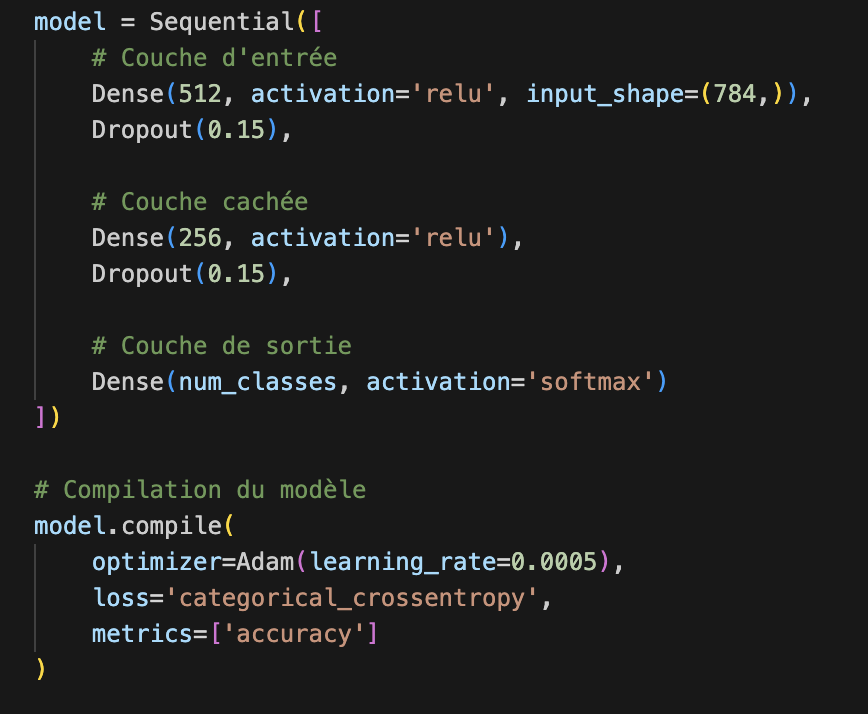
\includegraphics[width=0.5\textwidth]{figures/ArchiMLP.png}
\caption{Architecture du Perceptron.}
\label{fig:Architecture CNN Simple}
\end{figure}



\section*{Annexe 3: Architecture CNN Simple}
\label{sec:annexe3}
\begin{figure}[H]
\centering
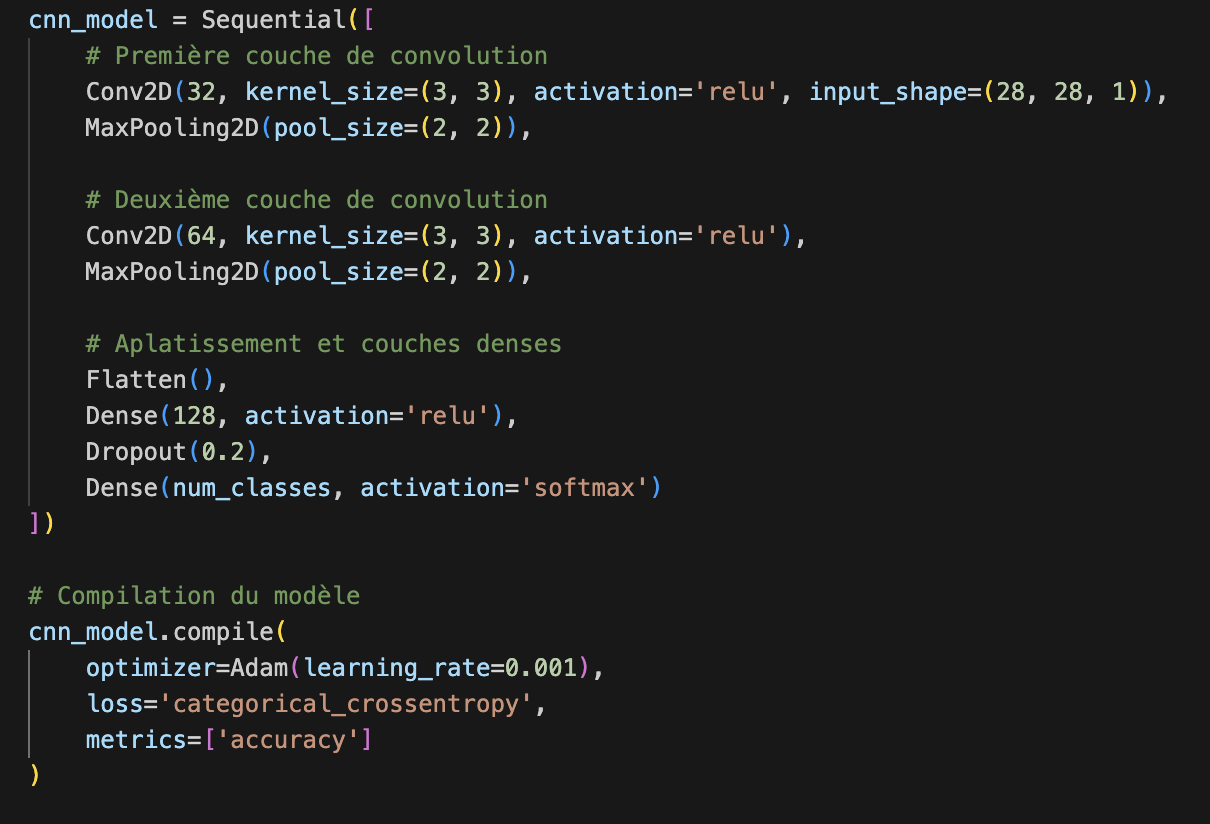
\includegraphics[width=0.5\textwidth]{figures/ArchiCNNSIMPL.png}
\caption{Architecture CNN Simple.}
\label{fig:Architecture CNN Simple}
\end{figure}




\section*{Annexe 4: Code source des principales fonctions}
\label{sec:annexe2}
\begin{itemize}
\item Prétraitement des données
\begin{figure}[H]
\centering
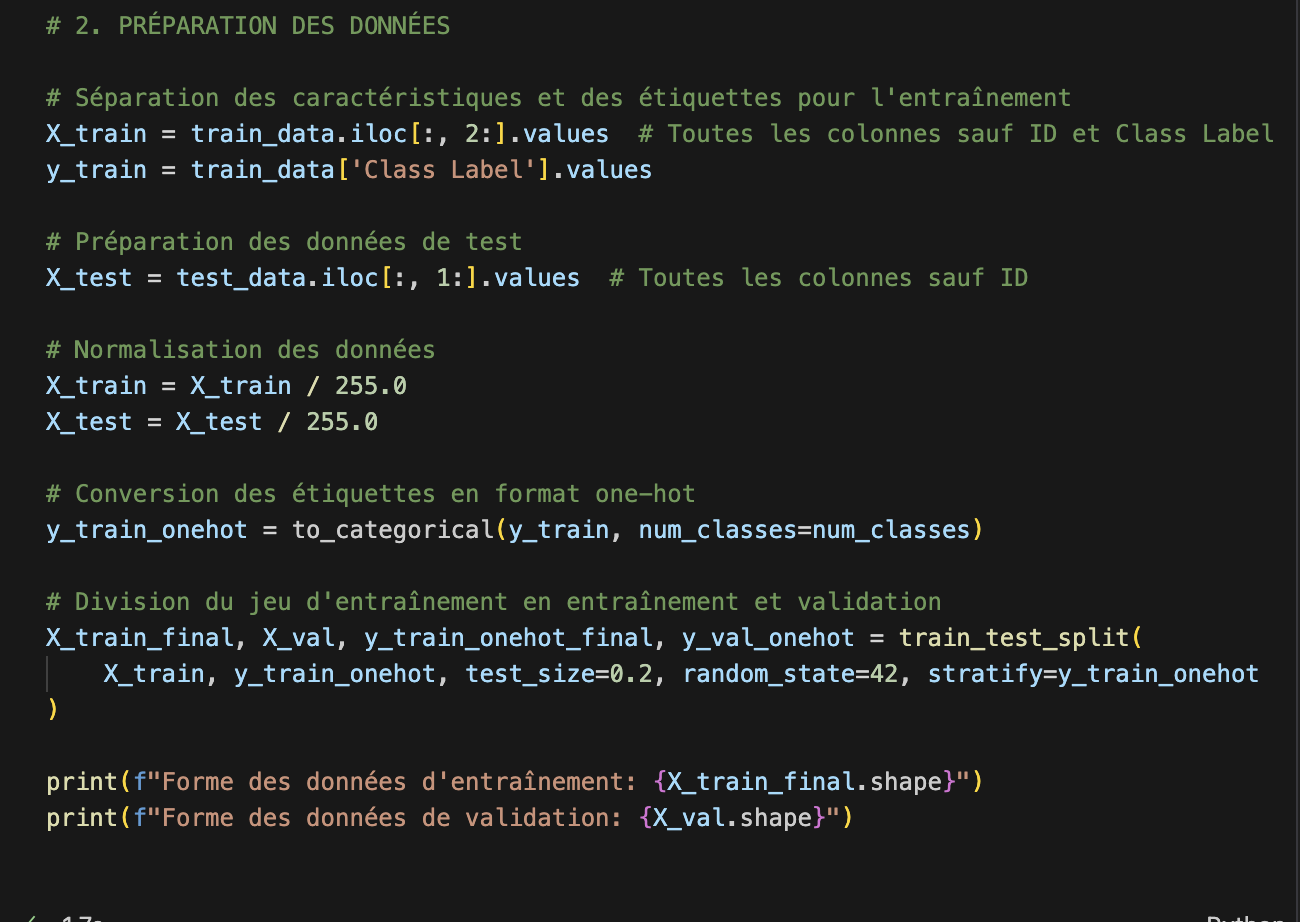
\includegraphics[width=0.5\textwidth]{figures/annexePre.png}
\caption{Code Pré traitement des données.}
\label{fig:Prétraitement des données}
\end{figure}
\item Visualisation des résultats
\begin{figure}[H]
\centering
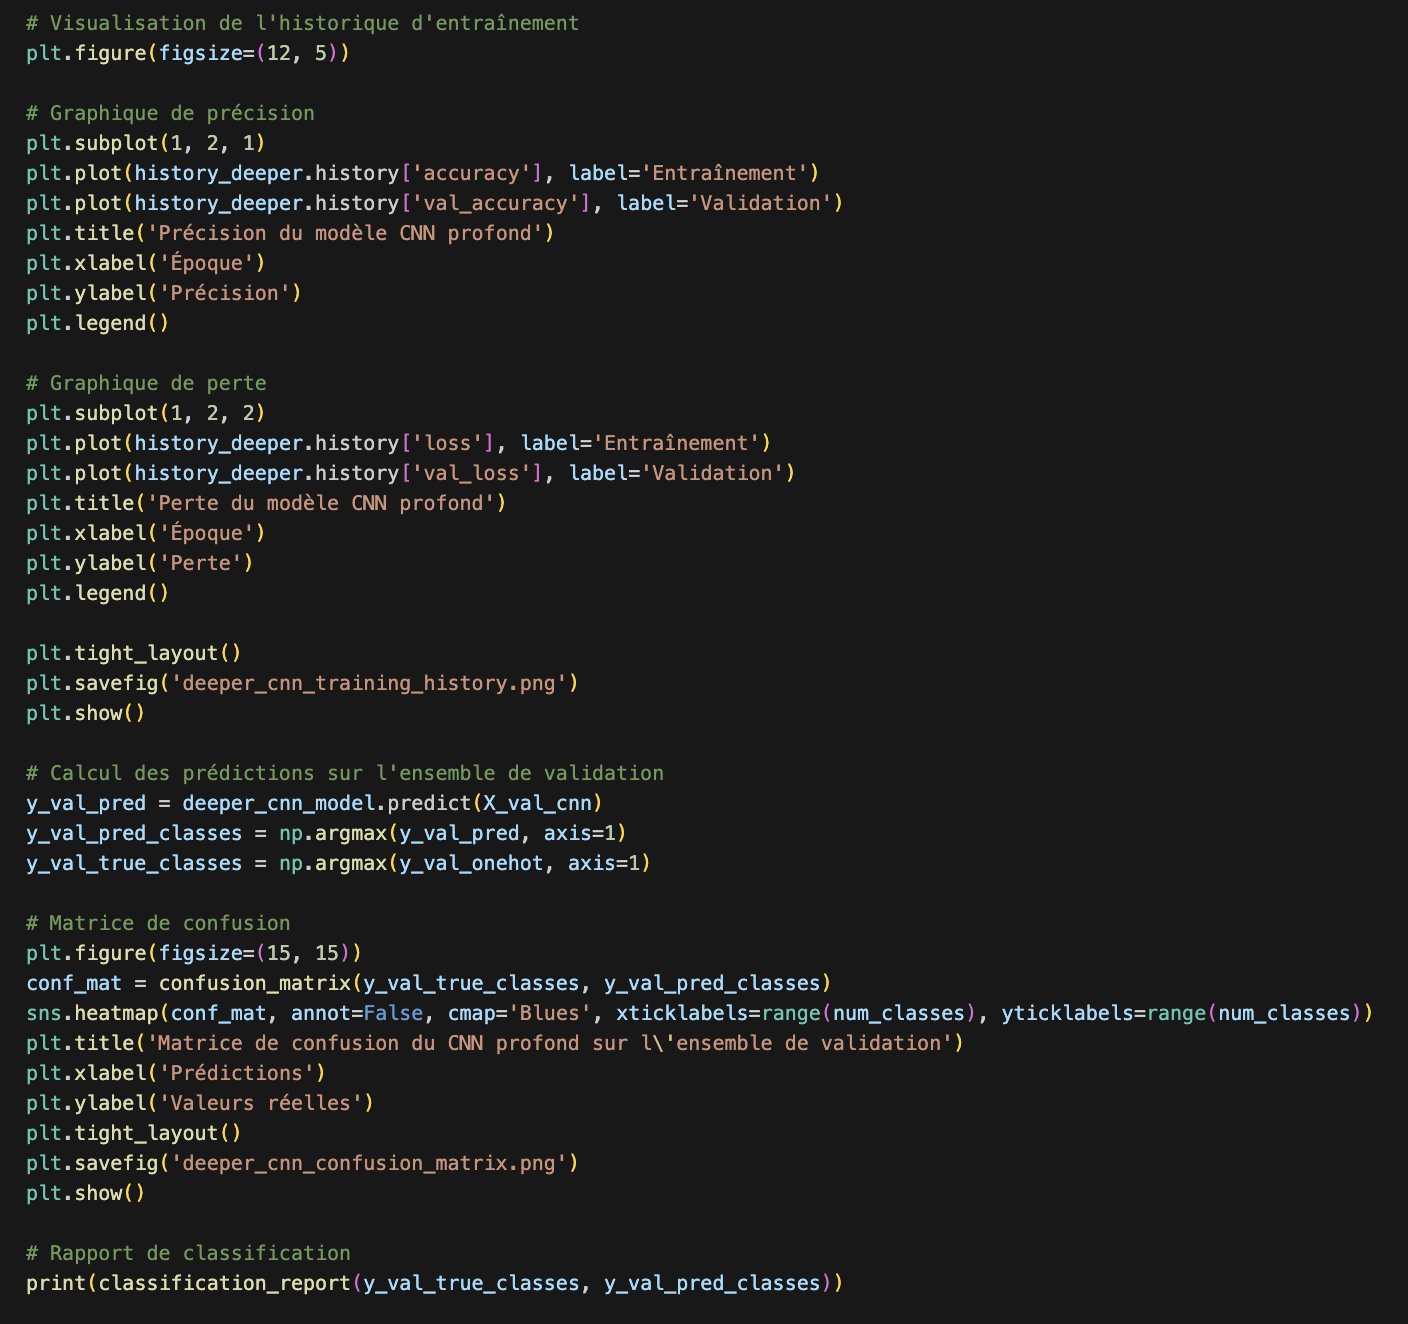
\includegraphics[width=0.5\textwidth]{figures/annexeVisua.png}
\caption{Code de visualisation des résultats.}
\label{fig:annexeVisua}
\end{figure}
\end{itemize}


\section*{Annexe 5: Annexe MLP}
\label{sec:annexe5}
\begin{itemize}
\item Précision et Perte du modèle
\begin{figure}[H]
\centering
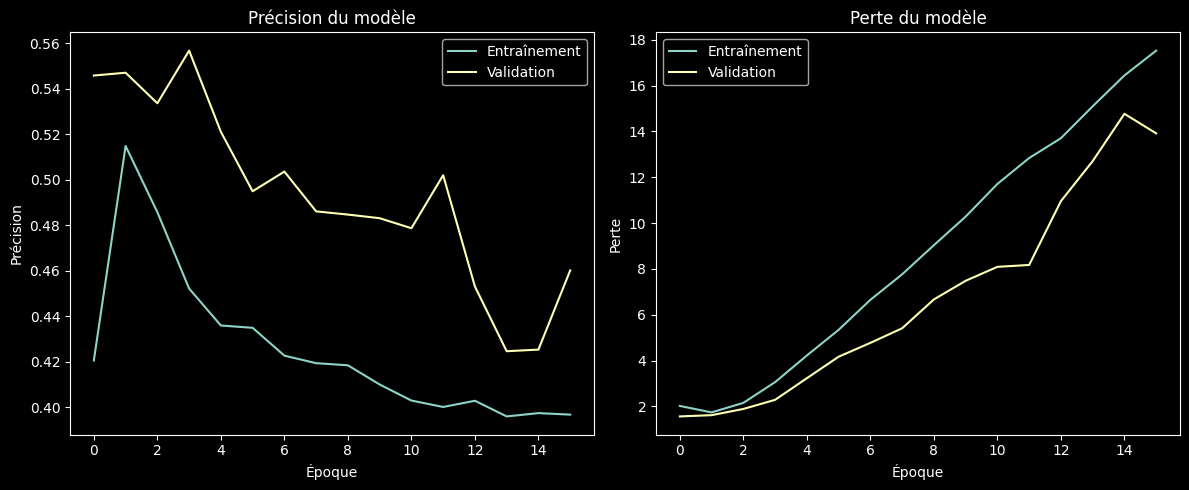
\includegraphics[width=0.5\textwidth]{figures/MLP1.png}
\caption{Courbe de précision et de perte.}
\label{fig:annexe5.1}
\end{figure}
\item Matrice de confusion
\begin{figure}[H]
\centering
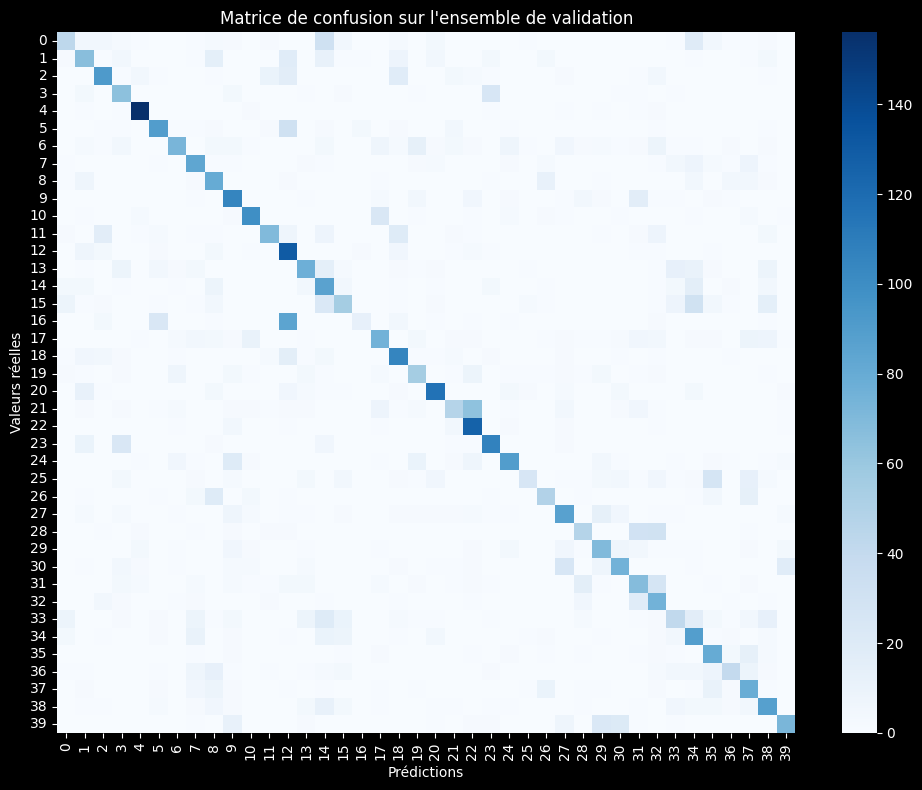
\includegraphics[width=0.5\textwidth]{figures/MLP2.png}
\caption{Matrice de confusion.}
\label{fig:annexe5.2}
\end{figure}
\item Résumé statistique du modèle
\begin{figure}[H]
\centering
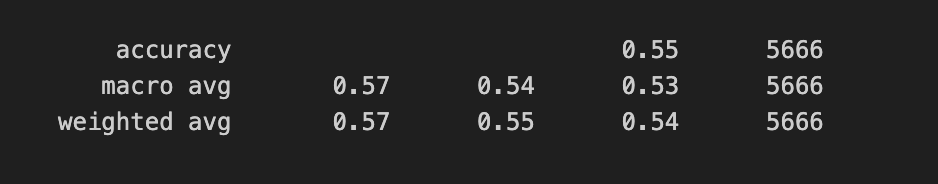
\includegraphics[width=0.5\textwidth]{figures/MLP3.png}
\caption{Résumé Statistique du modèle MLP.}
\label{fig:annexe5.3}
\end{figure}
\end{itemize}


\section*{Annexe 6: Modèle CNN Simple}
\label{sec:annexe6}
\begin{itemize}
\item Précision et Perte du modèle
\begin{figure}[H]
\centering
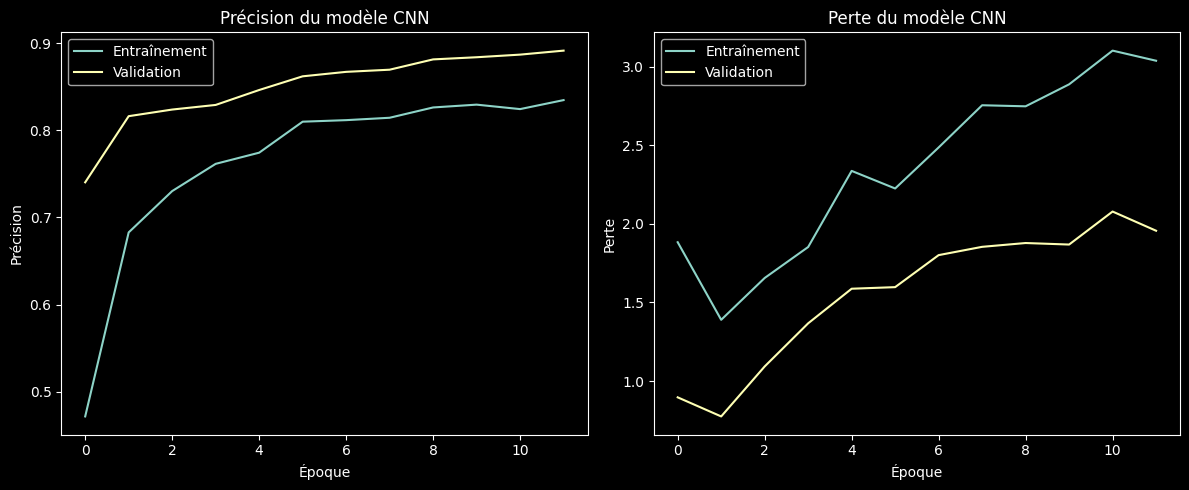
\includegraphics[width=1\textwidth]{figures/CNNSIMPLE1.png}
\caption{Courbe de précision et de perte.}
\label{fig:annexe6.1}
\end{figure}
\item Matrice de confusion
\begin{figure}[H]
\centering
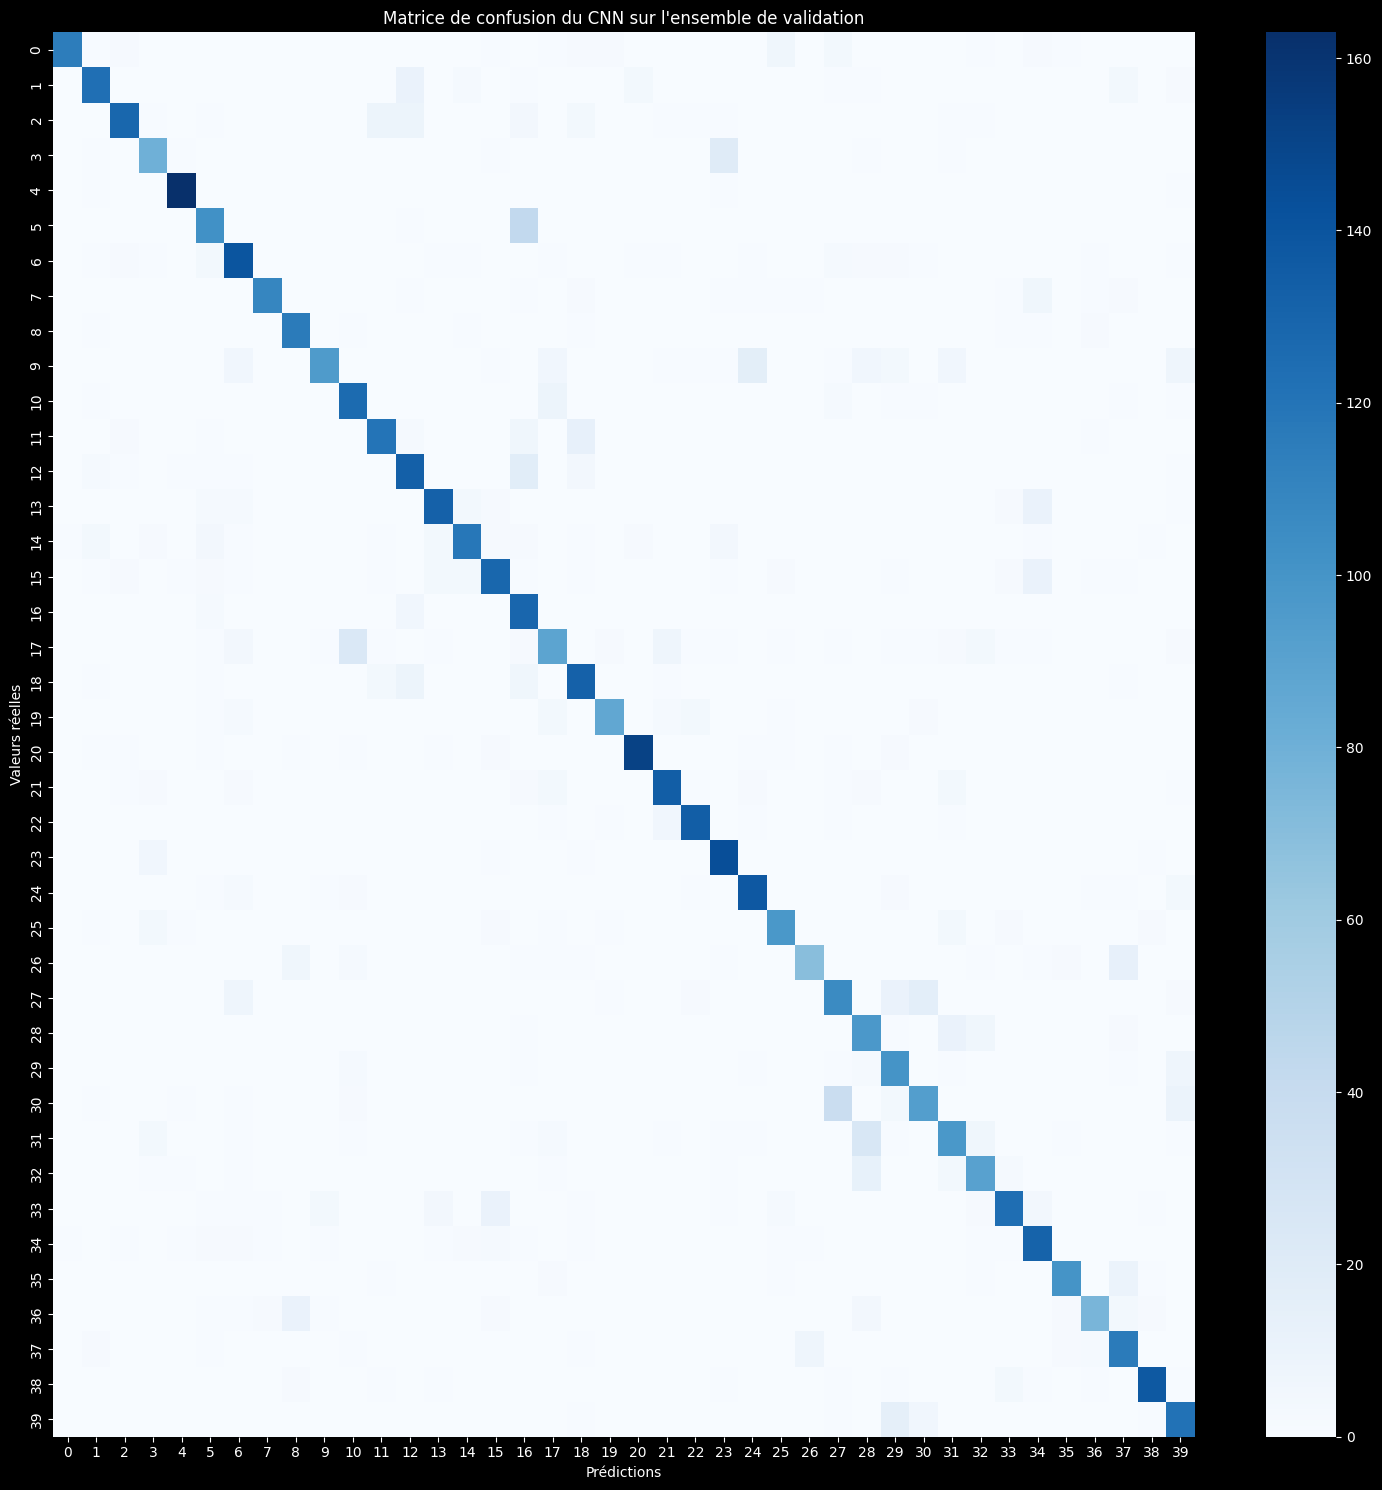
\includegraphics[width=0.5\textwidth]{figures/CNNSIMPLE2.png}
\caption{Matrice de confusion.}
\label{fig:annexe6.2}
\end{figure}
\item Résumé statistique du modèle
\begin{figure}[H]
\centering
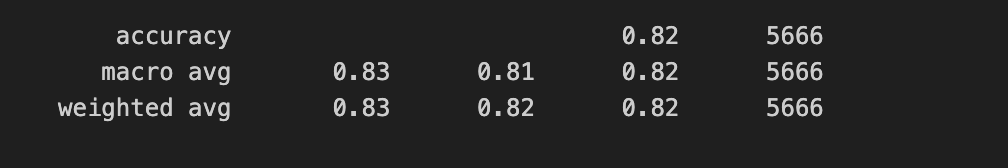
\includegraphics[width=0.5\textwidth]{figures/CNNSIMPLE3.png}
\caption{Résumé Statistique du modèle CNN Simple.}
\label{fig:annexe6.3}
\end{figure}
\end{itemize}



\section*{Annexe 7: Modèle CNN Profonde}
\label{sec:annexe7}
\begin{itemize}
\item Précision et Perte du modèle
\begin{figure}[H]
\centering
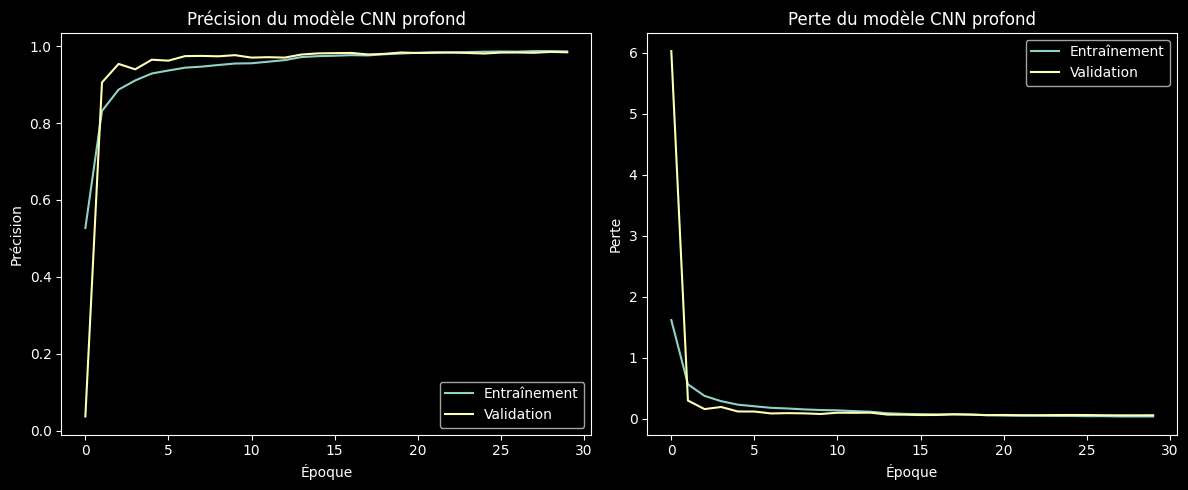
\includegraphics[width=1\textwidth]{figures/CNNPRO1.png}
\caption{Courbe de précision et de perte.}
\label{fig:annexe7.1}
\end{figure}
\item Matrice de confusion
\begin{figure}[H]
\centering
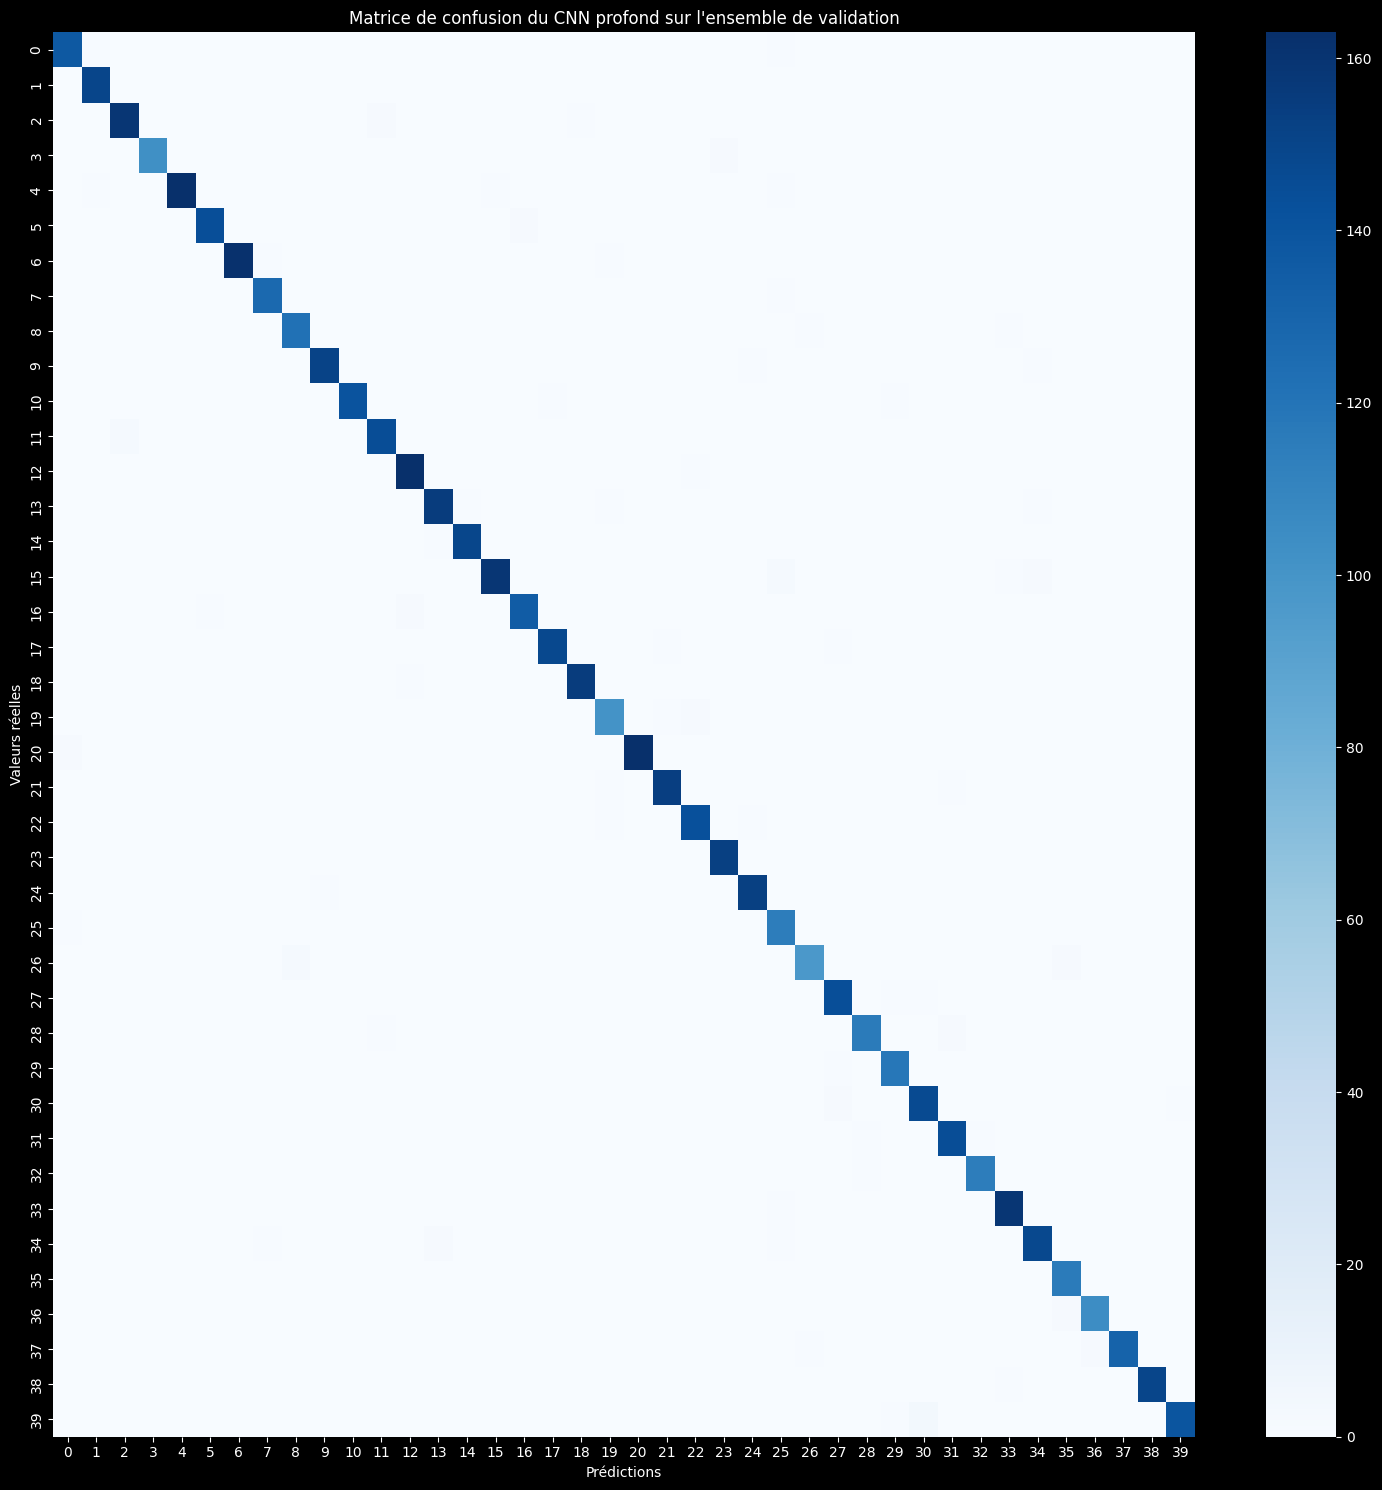
\includegraphics[width=0.5\textwidth]{figures/CNNPRO2.png}
\caption{Matrice de confusion.}
\label{fig:annexe7.2}
\end{figure}
\item Résumé statistique du modèle
\begin{figure}[H]
\centering
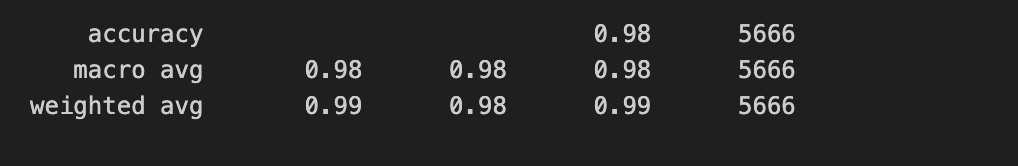
\includegraphics[width=0.5\textwidth]{figures/CNNPRO3.png}
\caption{Résumé Statistique du modèle CNN Profonde.}
\label{fig:annexe7.3}
\end{figure}
\end{itemize}


 
\addstarredchapter{Bibliographie}
\nocite{*}
\bibliographystyle{plainurl}
\bibliography{references}
\end{document}